\documentclass[]{elsarticle} %review=doublespace preprint=single 5p=2 column
%%% Begin My package additions %%%%%%%%%%%%%%%%%%%
\usepackage[hyphens]{url}

  \journal{European Economic Review} % Sets Journal name


\usepackage{lineno} % add

\usepackage{graphicx}
%%%%%%%%%%%%%%%% end my additions to header

\usepackage[T1]{fontenc}
\usepackage{lmodern}
\usepackage{amssymb,amsmath}
\usepackage{ifxetex,ifluatex}
\usepackage{fixltx2e} % provides \textsubscript
% use upquote if available, for straight quotes in verbatim environments
\IfFileExists{upquote.sty}{\usepackage{upquote}}{}
\ifnum 0\ifxetex 1\fi\ifluatex 1\fi=0 % if pdftex
  \usepackage[utf8]{inputenc}
\else % if luatex or xelatex
  \usepackage{fontspec}
  \ifxetex
    \usepackage{xltxtra,xunicode}
  \fi
  \defaultfontfeatures{Mapping=tex-text,Scale=MatchLowercase}
  \newcommand{\euro}{€}
\fi
% use microtype if available
\IfFileExists{microtype.sty}{\usepackage{microtype}}{}
\bibliographystyle{elsarticle-harv}
\ifxetex
  \usepackage[setpagesize=false, % page size defined by xetex
              unicode=false, % unicode breaks when used with xetex
              xetex]{hyperref}
\else
  \usepackage[unicode=true]{hyperref}
\fi
\hypersetup{breaklinks=true,
            bookmarks=true,
            pdfauthor={},
            pdftitle={An Independent European Macro? A History of European Macroeconomics through the Lens of the European Economic Review},
            colorlinks=false,
            urlcolor=blue,
            linkcolor=magenta,
            pdfborder={0 0 0}}
\urlstyle{same}  % don't use monospace font for urls

\setcounter{secnumdepth}{5}
% Pandoc toggle for numbering sections (defaults to be off)


% tightlist command for lists without linebreak
\providecommand{\tightlist}{%
  \setlength{\itemsep}{0pt}\setlength{\parskip}{0pt}}


% Pandoc citation processing
\newlength{\cslhangindent}
\setlength{\cslhangindent}{1.5em}
\newlength{\csllabelwidth}
\setlength{\csllabelwidth}{3em}
\newlength{\cslentryspacingunit} % times entry-spacing
\setlength{\cslentryspacingunit}{\parskip}
% for Pandoc 2.8 to 2.10.1
\newenvironment{cslreferences}%
  {}%
  {\par}
% For Pandoc 2.11+
\newenvironment{CSLReferences}[2] % #1 hanging-ident, #2 entry spacing
 {% don't indent paragraphs
  \setlength{\parindent}{0pt}
  % turn on hanging indent if param 1 is 1
  \ifodd #1
  \let\oldpar\par
  \def\par{\hangindent=\cslhangindent\oldpar}
  \fi
  % set entry spacing
  \setlength{\parskip}{#2\cslentryspacingunit}
 }%
 {}
\usepackage{calc}
\newcommand{\CSLBlock}[1]{#1\hfill\break}
\newcommand{\CSLLeftMargin}[1]{\parbox[t]{\csllabelwidth}{#1}}
\newcommand{\CSLRightInline}[1]{\parbox[t]{\linewidth - \csllabelwidth}{#1}\break}
\newcommand{\CSLIndent}[1]{\hspace{\cslhangindent}#1}

\usepackage{float}
\usepackage{booktabs}
\usepackage{longtable}
\usepackage{array}
\usepackage{multirow}
\usepackage{wrapfig}
\usepackage{colortbl}
\usepackage{pdflscape}
\usepackage{tabu}
\usepackage{threeparttable}
\usepackage{threeparttablex}
\usepackage[normalem]{ulem}
\usepackage{makecell}
\usepackage{xcolor}



\begin{document}


\begin{frontmatter}

  \title{An Independent European Macro? A History of European
Macroeconomics through the Lens of the European Economic Review}
    \author[1]{Aurélien Goutsmedt\corref{3}}
  
    \author[2]{Alexandre Truc}
  
      \address[1]{UCLouvain, ISPOLE. Collège Jacques Leclercq, Place
Montesquieu, 1/L 2.08.07, 1348 - Louvain-la-Neuve.}
    \address[2]{Université Côte d'Azur, CNRS GREDEG France.}
      \cortext[3]{Corresponding Author: aurelien.goutsmedt@uclouvain.be}
  
  \begin{abstract}
  Economics in Europe has encountered a process of internationalisation
  since the 1970s. To a certain extent, this internationalisation is
  also an `Americanisation' and many European departments and economics
  have adopted the standards of US economics, notably mathematical
  modelling, the use of econometrics, and the neoclassical theory as a
  modelling benchmark. Regarding this process, we can wonder if European
  economics has just been mimicking US economics since the 1970s, or if
  some European specialities have survived or emerged.

  In this article, we use topic modelling and bibliometric coupling to
  identify what have been some European specialities between 1969 and
  2002. We focus on one economics sub-discipline, macroeconomics, and we
  use the articles published in the European Economic Review and compare
  their bibliographic references and content to what has been published
  in the top 5 journals.
  \end{abstract}
  
 \end{frontmatter}

\hypertarget{introduction}{%
\section{Introduction}\label{introduction}}

In 1987 in the \emph{European Economic Review}, the director of the
Centre for Economic Policy Research, Richard Portes, attempted to assess
the ``state and status of economics in Europe''. He regarded ``the
standard of comparison {[}as{]} obvious: the United States, by far the
dominant producer'' (\protect\hyperlink{ref-portes1987}{Portes, 1987, p.
1329}). He then asked ``whether there is now any economics outside and
independent of the United States.'' (1330) He gave a list of the many
indices testifying of the US domination, ending it by the fact that
``the leaders of the economics profession in Europe were trained as
postgraduates in the United States. Many take from the US their
professional standards, their views of what are the interesting
problems, and their approaches to them''. (\emph{ibid.})

Indeed, since the early 1970s, economics in many Western European
countries had entered in a process of internationalisation
(\protect\hyperlink{ref-fourcade2009}{Fourcade, 2009, chap. 3} and 4;
\protect\hyperlink{ref-fourcade2006}{Fourcade, 2006}). To some extent,
such process was also a form of ``Americanisation''
(\protect\hyperlink{ref-coats1996}{Coats, 1996};
\protect\hyperlink{ref-goutsmedt2021}{Goutsmedt et al., 2021}):
professional and intellectual standards were progressively adopted in
European countries, mimicking the functioning of the US academic field.
English gradually spread as the dominant language in economics
(\protect\hyperlink{ref-sandelin1997}{Sandelin and Ranki, 1997}) and
publications in peer-review journals became the norm for assessing
research productivity. The organisation of international events were
encouraged to boost research centres visibility
(\protect\hyperlink{ref-cherrier2021}{Cherrier and Saïdi, 2021};
\protect\hyperlink{ref-goutsmedt2021}{Goutsmedt et al., 2021}). In terms
of content, the Americanisation of the discipline in Europe favoured the
intellectual standards that had become widespread in the US in the
postwar era (\protect\hyperlink{ref-morgan1998}{Morgan and Rutherford,
1998}): the use of mathematical economics and econometrics, and the
reliance on neoclassical theory as a benchmark for modelling.\footnote{Of
  course, this process of Americanisation did not go without conflicts:
  many ``local conflicts'' emerged between more ``nationally-trained''
  economists (generally locally trained) and ``internationally-trained
  economists'' who had been often trained in the US
  (\protect\hyperlink{ref-fourcade2006}{Fourcade, 2006}). These
  conflicts involved intellectual matters (for instance around the
  relevance of the neoclassical theory) as well as institutional issues,
  like the criteria to assess the quality of economists' work and thus
  to determine hiring and promotion.}

In parallel to this Americanisation, we can observe a process of
`Europeanisation': many initiatives from the first issue of the
\emph{European Economic Review} (EER) in 1969 to the creation of the
\emph{Economic European Association} (EEA) in 1984 promoted the
development of intellectual exchanges between European
economists---while obviously keeping US economics as a model. The
simultaneous spreading of US standards in Europe after the 1970s and the
promotion of a European economics transcending national traditions bring
us back to Portes's 1987 question: was there a possibility after the
1970s for the existence and persistence of a European tradition of
economics, relatively autonomous from the US profession?

Portes pointed out some European ``comparative advantages''
(\protect\hyperlink{ref-portes1987}{Portes, 1987, p. 1332}) even if some
of these European specialities had been pioneered by US economists. He
highlighted the dynamism in Europe of ``general equilibrium
theory{[},{]} social choice, duality, and the analysis of repeated
games'', ``international macroeconomic policy coordination'' or
``Non-Walrasian macroeconomics'' (\emph{ibid}.). Goutsmedt et al.
(\protect\hyperlink{ref-goutsmedt2021}{2021}) have also highlighted that
within the \emph{International Seminar on Macroeconomics} (ISoM), whose
proceedings were published annually in the EER, Disequilibrium
macroeconomics and large-scale macroeconometric modelling constituted
important rallying points until the mid-1980s for the European
economists involved in the ISoM.\footnote{Clarifying the label of
  non-walrasian macro here. Ref to backhouse and boianovsky}

The purpose of our article is to investigate this issue systematically
and quantitatively. Regarding the history of the EER and its importance
in the promotion of a European economics (see section
\ref{EER-creation}), we think that it constitutes a good proxy for
observing the emergence and persistence of `European specialities'. We
define specialities as widespread research topics \emph{(i)} distinct
from what US-based economists were doing, \emph{(ii)} adopted by many
European-based economists in different European countries, and
\emph{(iii)} bringing collaboration between different universities.
Using bibliometric coupling and topic modelling joined to more
qualitative content analysis, we identify European specialities from
1973 to 2002 (section \ref{european-specialities}).\footnote{{[}Could be
  revised depending on our final choices{]} The corpus we use (see
  section \ref{methods}) has very few abstracts between 1969 (the date
  of the creation of the EER) and 1972. Besides, there is no JEL code
  for EER articles before 1973, preventing us for identifying
  macroeconomics articles (see below). After 2002 and the creation of
  the \href{https://academic.oup.com/jeea}{\emph{Journal of the European
  Economic Association}}\emph{,} the EER was not the official journal of
  the EEA any more.}

The history of recent economics has mimicked the hierarchy of the
discipline by focusing mainly on US economists (and their ideas) or
institutions. Of course, some history of economics articles have dealt
with the peculiarities of economics in some European countries since the
1970s or with important European economists
(\protect\hyperlink{ref-benest2019}{Benest, 2019};
\protect\hyperlink{ref-maes2005}{Maes and Buyst, 2005}). However, our
goal here is to investigate this issue at the European level and to
understand if the internationalisation of the discipline since the 1970s
have been accompanied by the emergence of European specialities,
relatively independent of the US main topics and overcoming mere
national traditions. Besides, we use quantitative methods, as we think
that the latter are useful to get a general picture while limiting
biased choices and focus.\footnote{Indeed, it could be easy and tempting
  to pick such or such areas of study and find one or two important
  European economists working on it, to make it a European speciality.
  Even if they involve choices and interpretations, we think that the
  methods we use limit this risk}

However, we are focusing only on macroeconomics articles, mainly because
we think that such an investigation involved in-depth qualitative
\emph{and} qualitative analyses of these specialities and a relatively
good knowledge of the literature. A similar investigation on the whole
economic field would have been beyond our analytical capabilities.
Besides, macroeconomics constituted a substantial part of EER
publications, even representing almost half of all the articles in the
early 1980s (Figure \ref{fig:plot-jel}). Macroeconomics was also
instrumental in fostering collaborations between European economists as
the ``International Seminar on Macroeconomics'' testifies (see Section
\ref{rising-journal}). This article also relies on a unique dataset,
which has been constituted by merging the content of four different
institutional databases (see Section \ref{methods}).\footnote{The
  article is also accompanied by a detailed methodological
  \protect\hyperlink{appendix}{Appendix}.}

\begin{figure}[h]

{\centering \includegraphics[width=1\linewidth]{C:/Users/goutsmedt/Mon Drive/data/EER/pictures/Graphs/mean_jel} 

}

\caption{Share of Articles with at least one macroeconomics JEL code}\label{fig:plot-jel}
\end{figure}

\hypertarget{EER-creation}{%
\section{The Creation of the EER}\label{EER-creation}}

\hypertarget{the-birth-of-a-european-project}{%
\subsection{The Birth of a European
Project}\label{the-birth-of-a-european-project}}

In 1969, Jean Waelbroeck and Herbert Glejser, both from the
\emph{Université Libre de Bruxelles} (ULB), launched the \emph{European
Economic Review}. The new review was planned to be the official journal
of the European Scientific Association of Applied Economics (ASEPELT),
which had been created in 1961 by Waelbroeck and another ULB economist:
Etienne Kirschen. Before 1969, the association published in English a
bulletin gathering research in econometrics and mathematical economics
(\protect\hyperlink{ref-waelbroeck1969}{Waelbroeck and Glejser, 1969, p.
4}). The EER took up this torch by publishing the same type of research.
Articles had to be published in English, the new ``\emph{lingua franca}
of economics'' triggering the process of ``internationalisation of our
science'' as Waelbroeck and Glejser polemically stated in the
introduction of the first issue (\emph{ibid.}).

The fact that such a project was born in Belgium is no coincidence.
Indeed, the country displayed a high effervescence regarding the
internationalisation of the discipline. In 1966, Jacques Drèze had
established the Center for Operations Research and Econometrics (CORE)
at the \emph{Katholieke Universiteit Leuven} (before its split), on the
model of the Cowles Commission and the Carnegie Institute of Technology,
which Drèze had visited in the 1950s
(\protect\hyperlink{ref-duppe2017}{Düppe, 2017}).\footnote{KU Leuven was
  split in 1968 between a Flamish and a French-speaking part, the latter
  giving birth to the \emph{Université Catholique de Louvain} at
  Louvain-La-Neuve, where the CORE eventually moved in the mid-1970s.}
The CORE developed a research program around econometrics and
macroeconomic modelling and quickly stimulated the establishment of a
European research network of economists, notably through its large
visiting programme (\protect\hyperlink{ref-duppe2017}{Düppe, 2017};
\protect\hyperlink{ref-maes2005}{Maes and Buyst, 2005}). Encouraged by
Waelbroeck, the ULB department of economics joined the CORE in its first
years of existence (\protect\hyperlink{ref-maes2005}{Maes and Buyst,
2005, p. 79}).

The EER being a Belgian-centred initiative, Belgian institutions
represented one fourth of authors' affiliations in EER articles in the
first years (Figure \ref{fig:plot-authors}).\footnote{This is an
  approximation, as the affiliation per author is not available in our
  corpus and we only have the affiliations per article (see
  \protect\hyperlink{author-affiliation}{Appendix B.2.} for more
  details).} Nonetheless, the EER authorship became increasingly diverse
in the 1970s in terms of geographic affiliation. From the beginning, the
EER was conceived as a European project and the composition of the
editorial board testifies of it (Figure \ref{fig:plot-boards}).

\begin{figure}[h]

{\centering \includegraphics[width=1\linewidth]{C:/Users/goutsmedt/Mon Drive/data/EER/pictures/Graphs/EER_affiliations} 

}

\caption{Share of countries of authors' affiliations in EER publications (Top 10)}\label{fig:plot-authors}
\end{figure}

The EER was one of these crucial initiatives that contributed to the
development of intellectual exchanges between European based economists
(\protect\hyperlink{ref-goutsmedt2021}{Goutsmedt et al., 2021}). The
centrality of the journal was strengthened in 1984 when the European
Economic Association was created, and the EER established as the
official journal of the new association.

\begin{figure}[h]

{\centering \includegraphics[width=1\linewidth]{C:/Users/goutsmedt/Mon Drive/data/EER/pictures/Graphs/Board_affiliations} 

}

\caption{Share of countries in EER editorial boards (Top 10)}\label{fig:plot-boards}
\end{figure}

\hypertarget{rising-journal}{%
\subsection{A Rising European Journal}\label{rising-journal}}

Outside of offering a common platform for European economists, the
journal initial goal was also to encourage the promotion of a US style
of doing economics. An important dimension of the journal was thus the
progressive integration of US-based economists. The ``International
Seminar on Macroeconomics,'' co-organized by the French \emph{Ecole des
Hautes Etudes en Sciences Sociales} and the US National Bureau of
Economic Research, played a key role in that integration of US
economists, as the conference papers were published each year in a
special issue. It also likely contributed to make the journal known on
the other side of the Atlantic.

The share of US-based authors publishing in the journal grew steadily in
the 1970s and reached a third of all affiliations in the early 1980s
(Figure \ref{fig:plot-authors}). The increase of US economists
participation to the EER does not mean uniquely that more articles were
published by US authors, but also that the number of collaborations
between US- and European-based economists increased (Figure
\ref{fig:plot-collabs}). While there was no collaboration in the first
year of the journal, 10 percent of the articles published in 1980 mixed
institutions from the US and Europe.

\begin{figure}[h]

{\centering \includegraphics[width=1\linewidth]{C:/Users/goutsmedt/Mon Drive/data/EER/pictures/Graphs/Collab_strict} 

}

\caption{Patterns of collaboration between the United States and European countries in EER (noodle version)}\label{fig:plot-collabs}
\end{figure}

In the mid-1980s, the journal was thus a symbol of a more integrated
European economics, inspired by the US standards, as well as it was
attracting many US economists to publish in it. Its intellectual
influence similarly expanded and it became a major economic journal,
overcoming other important European journals in terms of bibliographic
citations (Figure \ref{fig:plot-eer-importance}). This trend was even
more significant in macroeconomics (Figure \ref{fig:plot-eer-macro})

\begin{figure}[h]

{\centering \includegraphics[width=1\linewidth]{C:/Users/goutsmedt/Mon Drive/data/EER/pictures/Graphs/EER_Importance_econ} 

}

\caption{Share of total citations from economics journal going to EER}\label{fig:plot-eer-importance}
\end{figure}

\begin{figure}[h]

{\centering \includegraphics[width=1\linewidth]{C:/Users/goutsmedt/Mon Drive/data/EER/pictures/Graphs/EER_Importance_macro} 

}

\caption{Share of total citations from macroeconomics articles going to EER}\label{fig:plot-eer-importance-macro}
\end{figure}

But has this whole process led to the total standardisation of a
European economics on the US model, or has it led to the development (or
persistence) of proper European specialities?

\hypertarget{european-specialities}{%
\section{Methods for Identifying European
Specialities}\label{european-specialities}}

The first step was to build our dataset. To identify European
specialities, we compare macroeconomics articles published in the EER
and in the Top-5 journals (\emph{American Economic Review},
\emph{Journal of Political Economy}, \emph{Econometrica},
\emph{Quarterly Journal of Economics}, \emph{Review of Economic
Studies}). Focusing on the Top 5 allows us to only get the most popular
and dominant trends in macroeconomics and thus to draw clearer
comparisons with what is published in the EER. Besides, the EER was
created with the intent to establish an elite leading journal for the
European community that would imitate the standards of US major
journals. The Top 5 thus seems an adequate benchmark to compare the EER
to.

We identify macroeconomics articles by using the former and new JEL
codes classifications (\protect\hyperlink{ref-jel1991}{JEL,
1991}).\footnote{See the complete list of all the JEL codes we have used
  in \protect\hyperlink{eer-top5-macro}{Appendix B.1.}.} Outside of JEL
codes data, we have used three different databases to collect different
types of information: outside of basic metadata (year of publication,
title, authors, \emph{etc.}), we have collected the list of
bibliographic references of the EER and Top-5 articles, the abstracts,
and authors affiliations.\footnote{Crossing databases has been necessary
  due to missing years and information in the different databases we
  have used (Web of Science, Scopus and Microsoft Academic Premier). See
  the \protect\hyperlink{corpus}{Appendix B.1.} for more details on the
  building of our dataset.} Then, we have conducted two different types
of analysis to identify European specialities.

\hypertarget{bibliographic-coupling}{%
\subsection{Bibliographic coupling}\label{bibliographic-coupling}}

Bibliographic coupling connects articles together depending on the
bibliographic references they share. We build different networks of EER
and Top-5 articles (the nodes of the network), connected together by a
weighted edge, depending on the number of references two articles share
together.\footnote{For more details on the measure of weights, see the
  \protect\hyperlink{network}{Appendix B.3.}.} We build networks on a
moving ten-year window (depending on the year of publication of the
articles). We thus have ALEX TO DO networks from the 1973-1982 period,
through 1974-1983, 1975-1984, \emph{etc.}, to the 1993-2002
period.\footnote{Due to missing JEL codes for EER before 1973, we are
  forced to begin with the 1973-1982 window.} For each network, we use
the Leiden algorithm (\protect\hyperlink{ref-traag2019}{Traag et al.,
2019}) to identify bibliographic clusters, that is groups of articles
that share many references in common, and few with articles outside
their cluster. Articles which belongs to the same cluster are more
likely to share cognitive content (e.g., sharing objects of study,
methods, results or theory) even if disagreeing
(\protect\hyperlink{ref-claveau2016}{Claveau and Gingras, 2016};
\protect\hyperlink{ref-goutsmedt2021}{Goutsmedt et al., 2021};
\protect\hyperlink{ref-truc2021}{Truc et al., 2021}). Finally, we test
the similarity of the clusters two by two for successive time windows,
and merge clusters from different windows together when they are
sufficiently close.\footnote{See the
  \protect\hyperlink{network}{Appendix B.3.} for details on the merging
  criteria and summary information.}

This process allows us to obtain dynamic clusters Indeed, citation
patterns are highly dependent of the date of publication of an article:
scholars tend to cite more recent works. Consequently, for large time
window, clusters would likely be determined mainly by the publication
year, rather than by what they are talking about.\footnote{In other
  words, articles would be grouped together depending on the year of
  their publication and the clusterisation of the network would not say
  much of the economic content articles grouped together would share.}
By taking small time windows and then by merging communities in
different windows together, we avoid this problem and are able to
identify communities over longer period of time. We identify a total of
ALEX TO DO communities but only ALEX TO DO are \emph{(i)} present in at
least two networks (i.e.~two time windows) and \emph{(ii)} represent
more than 5 percent of the nodes of at least one of the network they
belong.\footnote{See table footnote}

A set of indicators allows us to understand what these clusters are
about---e.g.~the words used in abstracts and titles, the recurrent
authors and the most cited references. These indicators help us to name
the clusters. For each cluster, we calculate the difference between the
mean of the cluster articles published in the EER and the same mean for
the Top 5. We do the same for the articles published by European-based
economists only, and those published by US-based economists only
{[}PRECISE METHOD{]}. These two differences inform us on what are the
most `Europeans' clusters, meaning those where relatively more articles
are published in the EER by European-based economists.\footnote{Our
  assumption is that the content of articles published in the Top 5 by
  European economists could be more largely influenced by the standards
  of Top 5 journals and of US macroeconomics, and thus could be less
  representative of European economics than the articles published in
  the EER.} The figure \ref{fig:plot-community-diff} display the
position of each cluster relatively to these two differences. When we
sum the two differences, we have a synthetic indicator of how much a
cluster is European.

\begin{figure}[h]

{\centering \includegraphics[width=1\linewidth]{C:/Users/goutsmedt/Mon Drive/data/EER/pictures/Graphs/Communities_europeanisation_colored} 

}

\caption{The most European communities}\label{fig:plot-community-diff}
\end{figure}

\hypertarget{topic-modelling}{%
\subsection{Topic Modelling}\label{topic-modelling}}

Topic modelling is a non-supervised machine learning method which
associates \emph{(i)} the \emph{ngrams} contained in a corpus to
\emph{k} topics and \emph{(ii)} the documents of the corpus to the same
\emph{k} topics.\footnote{From the documents of our corpus, we extract
  (or `tokenise') unique words (or unigrams), bigrams and trigrams. Stop
  words and other uninformative words are excluded and all words are
  `lemmatised'. See the \protect\hyperlink{topic}{Appendix B.4.} for
  more details on the preprocessing steps we use.} We have used a
variant of the Latent Dirichlet Allocation model with the Correlated
Topic Model (\protect\hyperlink{ref-blei2007}{Blei and Lafferty, 2007}).
The number of topics \emph{k} is chosen by the modellers: after
assessing quantitatively and qualitatively different models, we choose
to run the model with 50 topics.\footnote{The
  \protect\hyperlink{topic}{Appendix B.4.} gives more details on the
  different models we have tested and how we have set the number of
  topics.} For each topic, we can look at the word with the highest
`FREX' value (\protect\hyperlink{ref-bischof2012}{Bischof and Airoldi,
2012}).\footnote{FREX is the weighted harmonic mean of the terms' rank
  regarding exclusivity and frequency scores. Exclusivity is a measure
  of how much a term is frequent in a topic in comparison to its
  frequency in others. In other words, a good topic model is a model
  where the words in topics are frequently used, but each topic can be
  easily dinstinguished from others, for the words associated to this
  topic are scarce in other topics.} The Table \ref{tab:summary-topics}
displays the words with the highest FREX value for each topic.

Similarly to what we do for bibliometric coupling, we are interested in
the topics characteristics regarding the publications (EER \emph{vs.}
Top 5) and the countries of affiliations of the authors (the US
\emph{vs.} European countries). As each article has a `rate of
belonging' to each topic (the \emph{gamma} value), we are able, for each
topic, to compute the difference in the means of \emph{gamma} values for
(i) articles published in the EER and articles published in the Top 5
and (ii) articles written by US-based authors and those written by
European-based authors. The resulting two differences are the
coordinates of the 50 topics in Figure \ref{fig:plot-topic-diff}. When
we sum the two differences, we have an indicator of how much a topic is
a European topic.

\begin{figure}[h]

{\centering \includegraphics[width=1\linewidth]{C:/Users/goutsmedt/Mon Drive/data/EER/pictures/topic_modelling/logratio_diff_plot} 

}

\caption{Topic Prevalence over journals (Difference of Means)}\label{fig:plot-topic-diff}
\end{figure}

\hypertarget{why-mixing-the-two-methods}{%
\subsection{Why mixing the two
methods?}\label{why-mixing-the-two-methods}}

To identifies specialties in a corpus, the existing literature usually
use bibliographic information and network analysis (topology-based
approach) or textual information and topic modeling (topic-based
approach). In the first case, articles that share the same bibliographic
informations (e.g., same references) are considered similar and part of
the same specialties (\protect\hyperlink{ref-claveau2016}{Claveau and
Gingras, 2016}). In the second case, using abstracts or full-text,
topics are assigned to individual articles, and specialties are
identified are derived from these topics
(\protect\hyperlink{ref-ambrosino2018}{\textbf{ambrosino2018?}}). These
two approaches use very different information (bibliographic information
vs text), and very different techniques (network analysis and cluster
detection vs probabilistic natural language processing).

In the informetrics literature, one can find some attempts to combine
both approaches (\protect\hyperlink{ref-ding2011}{\textbf{ding2011?}};
\protect\hyperlink{ref-li2012}{\textbf{li2012?}};
\protect\hyperlink{ref-yan2012}{\textbf{yan2012?}};
\protect\hyperlink{ref-mao2017}{\textbf{mao2017?}}), but it has never
been done in the economics literature. For the present article, we
propose to do so by using the two types of analysis jointly to identify
European specialties. The heterogeneous nature of both approaches
provide different advantages when used together.

First, both approaches give different information and are complementary.
Topology-based approach generally identify communities, while
topic-based approached identify topics. Communities and topics are often
considered intertwined: a community can have multiple topics, and a
given topic can be tackled by different communities
(\protect\hyperlink{ref-ding2011}{\textbf{ding2011?}};
\protect\hyperlink{ref-yan2012}{\textbf{yan2012?}}). For example, a
community of co-authors can cover different topics (e.g., a tight
network of microeconomists discussing health and education) while
different communities can cover similar topics (e.g., sociologists and
economists discussing health but never co-authoring papers). Topic
modeling can reveal heterogeneity of topics in a given community, while
network analysis can reveal the bibliographic or co-authoring network
that structure the same research topic. Using both approaches give a
more exhaustive picture of the forces that structure economics research.
Inversely, using both methods that can also reveal homogeneity, when
communities and topics overlaps, then it sends a stronger signal that a
community has a specific identity, is tightly knit and well-recognized.

A second advantage of using both methods is that they use different
techniques and data sources. Bibliographic and textual data from
scientific publications have imperfections. Publications before the
1970s do not always have abstracts, and authors can make mistakes when
referencing articles that lead to imperfect identification of
bibliographic data. Similarly, from a technical point of view, both
approaches are relatively recent, and the best algorithms/models used
suffer from analytical limits and are evolving very rapidly (e.g., see
(\protect\hyperlink{ref-zhang2020}{\textbf{zhang2020?}}) for community
detection). Using both approaches jointly can help triangulate results
and both methods can compensate for some of the weaknesses of the other.

\hypertarget{a-broad-picture-of-european-specialities}{%
\section{A Broad Picture of European
Specialities}\label{a-broad-picture-of-european-specialities}}

The purpose of our method is to identify different types of literature
that are in average more associated to the EER and to articles written
by European-based authors. In this section, we get a general idea of the
different specialities emerging from bibliometric coupling and topic
modelling analyses. In the two next sessions, we will sketch a more
encompassing portrait of the evolution of European macroeconomis from
the late 1970s to the late 1990s, while leaving aside some of the
specialities identified.

First, the two methods allow us to understand what European
macroeconomics \emph{was not}. A first consistent finding between the
two methods is that the literature about the life-cycle and permanent
income hypotheses, influenced by Friedman
(\protect\hyperlink{ref-friedman1957}{1957}) and Hall
(\protect\hyperlink{ref-hall1978b}{1978}), was far from popular for
European economists.\footnote{See communities ``Intergenerational model,
  Savings \& Consumption'' and ``Permanent Income and Life-Cycle
  Hypotheses'', as well as topics 12 and 14.} Heterogeneity was a
central issue for this literature (see Cherrier et al, this issue). Also
``less European'' are the contributions about the demand for money (for
which Baumol (\protect\hyperlink{ref-baumol1952}{1952}) and Friedman and
Schwartz (\protect\hyperlink{ref-friedman1963}{1963}) were central
references) as well as the ``new classical monetary theory''
(\protect\hyperlink{ref-hoover1988}{Hoover, 1988, chap. 6}) of the 1970s
inspired by Sargent's, Bryant's and Wallace's works (see for instance
Bryant and Wallace (\protect\hyperlink{ref-bryant1979}{1979}) or Sargent
and Wallace (\protect\hyperlink{ref-sargent1982}{1982})) or the more
recent ``New Monetarist Economics'' of Kiyotaki and Wright
(\protect\hyperlink{ref-kiyotaki1989}{1989}), Kiyotaki and Wright
(\protect\hyperlink{ref-kiyotaki1993}{1993}), and Trejos and Wright
(\protect\hyperlink{ref-trejos1995}{1995}; see
\protect\hyperlink{ref-frasser2020}{Frasser, 2020, chap. 2}, for an
historical reconstruction of this literature).\footnote{See communities
  ``Monetary Economics \& Demand for Money'' and ``New Theory of Money:
  Search, Bargaining\ldots{}'', and, even if it is not as
  ``non-European'' as the two others, the community ``Demand for
  Money''. For topics, see topic 2 on the demand for money and money
  supply, which is one of the most non-European topic, but also topic 19
  on demand for money and term structure of interest rates, influenced
  notably by Fama (\protect\hyperlink{ref-fama1975}{1975}).} The new
classical monetary theory of the 1970s is described by Hoover
(\protect\hyperlink{ref-hoover1988}{1988, p. 111}) as the research for
``microfoundations for the theory of money consistent with general
equilibrium and individual optimization'' promoted by new classical
economists (Lucas, Sargent, Wallace, etc.). More generally, it appears
that the works of new classical economists that contributed to reshaping
macroeconomics in the late 1970s and early 1980s, and that are so
central in many history of macroeconomics
(\protect\hyperlink{ref-devroey2016}{De Vroey, 2016}), were less
influential in Europe at the time. Articles like Lucas
(\protect\hyperlink{ref-lucas1972}{1972}), Lucas
(\protect\hyperlink{ref-lucas1973}{1973}), Barro
(\protect\hyperlink{ref-barro1974}{1974}), Sargent and Wallace
(\protect\hyperlink{ref-sargent1975}{1975}), Sargent and Wallace
(\protect\hyperlink{ref-sargent1976}{1976}) or Barro
(\protect\hyperlink{ref-barro1976}{1976}) were constantly undercited by
European-based macroeconomists in comparison to US economists in the
1970s and 1980s (see Figure \ref{fig:plot-new-classical}).\footnote{We
  have to wait 1982-1988 to see some new classical contributions cited
  as much by Europeans as by US economists. The integration of these
  contributions obviously took some time in Europe and lagged behind the
  US.} This is consistent with the fact that European macroeconomists
favoured in the late 1970s and early 1980s an alternative
``microfoundational programme''
(\protect\hyperlink{ref-hoover2012}{Hoover, 2012}) with disequilibrium
theory and non-walrasian macroeconomics (see Section
\ref{disequilibrium}).

\begin{figure}[h]

{\centering \includegraphics[width=1\linewidth]{C:/Users/goutsmedt/Mon Drive/data/EER/pictures/graphs/g2_over_citations} 

}

\caption{Citation of new classical works by European economists relatively to US-based economists}\label{fig:plot-new-classical}
\end{figure}

Second, the EER appeared as a more welcoming support for international
macroeconomics. All clusters and topics dealing with this kind of issues
are relatively over-represented in the EER (except one small topic on
gold standard and dollar reserves), and many topics are also
over-represented by European authors (see Figure
\ref{fig:plot-community-diff} and \ref{fig:plot-topic-diff}). Topics and
clusters on the political economy of central banking (see Section
\ref{political-economics}) and on unemployment (relying notably on
Pissarides (\protect\hyperlink{ref-pissarides1990}{1990}), Mortensen and
Pissarides (\protect\hyperlink{ref-mortensen1994}{1994}) and Layard et
al. (\protect\hyperlink{ref-layard1991a}{1991})) are also
over-represented both for EER and European authors.\footnote{See the
  ``Political Economics of Central Banks'' community and topic 8 for the
  first; and community ``Theory of Unemployment \& Job Dynamics'' and
  topic 37 for the second.} Lastly, our analyses make also appear a
proper European approach of time series and econometrics even if in a
large part a UK speciality: the ``LSE approach'' of David Hendry and his
colleagues (\protect\hyperlink{ref-qin2013a}{Qin, 2013, chap. 4}) and
the treatment of the cointegration issue.\footnote{See topic 46 and the
  community ``Business Cycles, Cointegration \& Trends''.}

The detailed analysis of clusters and topics offer a general panorama of
the different issues, methods and theoretical questions investigated by
European macroeconomists, in comparison to the US
macroeconomics.\footnote{See supplementary files for more information.}
However, this only gives us a fragmented (and for now a-historical)
picture of European macroeconomics. In the two last sections, we try to
draw a more unified picture of the evolution of European macroeconomics
between the mid-1970s and the late 1990s. Even if leaving aside some
identified specialities, we consider that two dynamics help to
understand the interaction between European and US macroeconomics, how
European macroeconomics distinguished itself, as well as how it has
transformed itself since the 1970s. Non-Walrasian macroeconomics or
disequilibrium theory represented in the 1970s and 1980s a theoretical
unifying research program for European macroeconomics.\footnote{Footnote
  on the label.} However it has progressively lost its influence after
the mid-1980s (see Section \ref{Disequilibrium}). If it did not
constitute a similar theoretical program, it appears to us that, in the
1990s, political economy played a similar role, constituting a European
speciality touching to many different economic problems (see Section
\ref{political-economics}).

\hypertarget{disequilibrium}{%
\section{Disequilibrium theory as a landmark for European
macroeconomics}\label{disequilibrium}}

Disequilibrium theory constituted an important but often forgotten step
in the history of macroeconomics
(\protect\hyperlink{ref-backhouseboianovski2013}{Backhouse and
Boianovski, 2013}; \protect\hyperlink{ref-plassard2021}{Plassard et al.,
2021}). It contributed significantly to the renewal of interest for the
research for microfoundations in macroeconomics in the 1970s (see
\protect\hyperlink{ref-duartelima2012a}{Duarte and Lima, 2012} for a
history of microfoundations in macroeconomics). Anchored in the general
equilibrium theory (GET) tradition and influenced by the work of
Patinkin, Clower and Leijonhufvud, disequilibrium theory explored the
impact of non-walrasian price-setting (i.e.~without \emph{tatonnement}),
fix-price and quantity rationing on macroeconomic outcomes. It
constituted an alternative to new classical contributions and the
``representative-agent microfoundational program'' of Lucas and Sargent
(\protect\hyperlink{ref-hoover2012}{Hoover, 2012}; see also
\protect\hyperlink{ref-renault2020a}{Renault, 2020}). Even if Barro and
Grossman's (\protect\hyperlink{ref-barro1971}{1971}) article was
fundamental in the popularisation of disequilibrium macroeconomics, the
research program was anchored in Europe, notably in France and Belgium
{[}Goutsmedt et al. (\protect\hyperlink{ref-goutsmedt2021}{2021});
Plassard and Renault, this issue{]}.\footnote{Appendix also displays
  some statistics on countries and institutions for each cluster and
  topic.}

It is quite clear from our bibliometric analysis that the
``Disequilibrium and Keynesian economics'' cluster constituted the most
significant cluster associated to the EER and and developed by European
economists. This cluster also integrates other ``alternative research
lines'' to Lucas's research program
(\protect\hyperlink{ref-devroey2016}{De Vroey, 2016, chap. 14}), like
Azariadis's (\protect\hyperlink{ref-azariadis1975}{1975}) implicit
contract model, Hart's (\protect\hyperlink{ref-hart1982}{1982})
imperfect competition model or Diamond's
(\protect\hyperlink{ref-diamond1982}{1982}) search model. It testifies
that in the late 1970s and in the 1980s, some connections existed
between US and European macroeconomists regarding the renewal of
theoretical macroeconomics and the search for microfoundations, and the
opposition to new classical macroeconomics. The topic modelling analysis
allows us to observe how widespread disequilibrium theory was for
European macroeconomics in the 1980s and how it unified the treatment of
different macroeconomic issues.

First of all, disequilibrium macroeconomics contributed to the
persistence of a dynamic research program around GET issues and part of
the literature ``arose out of the internal problems within general
equilibrium theory''
(\protect\hyperlink{ref-backhouseboianovski2013}{Backhouse and
Boianovski, 2013, p. 105}), notably the need to break with
\emph{tatonnement} and to build GET model with agents setting prices in
the model.\footnote{See topic 11.} But quickly, disequilibrium
macroeconomics also appeared as an important framework to deal with the
explanation of the current stagflation in the 1970s
(\protect\hyperlink{ref-backhouseboianovski2013}{Backhouse and
Boianovski, 2013, chap. 8}). Malinvaud's \emph{Theory of Unemployment
Reconsidered} (\protect\hyperlink{ref-malinvaud1977}{1977}) was a
decisive step in this direction by developing the opposition between
``Keynesian unemployment'', caused by excess supply in both goods and
labour markets, and ````classical unemployment'', triggered by excess
demand for goods, but excess supply in the labour market (involving that
real wages were too high).\footnote{Malinvaud
  (\protect\hyperlink{ref-malinvaud1977}{1977}) proposed a third regime,
  ``repressed inflation'' due to excess demand in both markets.} The oil
shock of 1973 and the simultaneous decrease of productivity explained
the apparition of a classical unemployment in the 1970s. The big issue
for adherents to this three regimes approach thus became to be able to
assess which part of European unemployment was due to Keynesian or to
classical unemployment.

This framework to think about unemployment and the stagflation has been
used, discussed, or at least mentioned in many important works for
European macroeconomics in the 1980s.\footnote{``Important'' means here
  highly cited by European economists in one or several cluster or
  topic.} Drèze and Modigliani (\protect\hyperlink{ref-dreze1981}{1981})
discussed in the EER the ``current state of underemployment in Belgium''
by analysing the trade off between real wages and employment in the
context of a small open economy (2). Drèze and Modigliani explained that
they mixed the possibility of classical unemployment, inspired by
Malinvaud (\protect\hyperlink{ref-malinvaud1977}{1977}), and Modigliani
and Padoa-Schioppa's argument that, ``in an open economy, external
balance implies a constraining relationship between the levels of real
wages and employment'' (2). Similarly, Malinvaud's framework was linked
in the early 1980s to the debate, often taking place in the EER, about
the ``wage gap'', that is the assessment of whether real wages were too
high (a positive wage gap) or too low. Bruno and Sachs were central
characters in this debate and relied explicitly on Malinvaud's
framework.\footnote{Bruno and Sachs's
  (\protect\hyperlink{ref-brunosachs1985}{1985}) of their late 1970s and
  early 1980s work constituted an highly cited resource for European
  macroeconomists (see also
  \protect\hyperlink{ref-goutsmedt2021}{Goutsmedt et al., 2021, sec.
  3}).}

Outside of unemployment and the stagflation issue, disequilibrium theory
was also extended to other macroeconomic issues. For instance, Avinash
Dixit, when at University of Warwick, extended Clower's dual decision
hypothesis and Malinvaud's framework to international trade theory
(\protect\hyperlink{ref-dixit1978}{Dixit, 1978, p. 393}). It gave the
basis to Dixit for promoting a ``more satisfactory model of the balance
of trade'' than Frenkel and Johnson's
(\protect\hyperlink{ref-frenkel1976}{1976}) monetary approach which
``assumes instantaneous attainment of Walrasian equilibrium in commodity
and labour markets'' (\protect\hyperlink{ref-dixit1978}{Dixit, 1978, p.
393}). Dixit's model would form the basis for some parts of Dixit and
Norman's book on the \emph{Theory of International Trade}
(\protect\hyperlink{ref-dixit1980}{Dixit and Norman, 1980}), which
constituted an important reference for European economists working on
international trade.\footnote{See topic 39.}

Disequilibrium theory constituted a significant part of the research
undertaken by European macroeconomists in the late 1970s and early
1980s, and did not limit to the GET, but also represented a unifying
framework to deal with different macroeconomic issues (unemployment,
stagflation, stabilization policies, international trade, etc.). This
centrality is also visible through the fact that many macroeconomists
had to position themselves in comparison to disequilibrium theory, and
notably to the Keynesian versus classical unemployment framework. In May
1985 was held a conference in Sussex about European unemployment,
published in \emph{Economica} the next year.\footnote{On this episode,
  see Backhouse, Forder and Laskaridis, as well as Plassard and Renault,
  both in this issue.} Macroeconomists from different countries
presented their analyses of European or national unemployment. While
Sneessens and Drèze estimated a ``two-market macroeconomic rationing (or
disequilibirum) model of the economy
(\protect\hyperlink{ref-sneessens1986}{Sneessens and Drèze, 1986, p.
S97}), Malinvaud (\protect\hyperlink{ref-malinvaud1986}{1986}) proposed
a more descriptive analysis to explain the rise of unemployment in
France, even if he claimed some proximity with Sneessens and Drèze
formalisation in the same issue. Malinvaud discussed some determinants
of''the classical component of unemployment''
(\protect\hyperlink{ref-malinvaud1986}{Malinvaud, 1986, p. S216}), but
also criticised the use of Phillips curve with a non-accelerating
inflation rate of unemployment (NAIRU) to deal with the causes of
unemployment. To the contrary, NAIRU was central in the model proposed
by Layard and Nickell to discuss unemployment in Britain and they
claimed that the ``labour demand function that we use cuts through the
fruitless debate now raging (especially in Europe) as to whether current
unemployment is `classical' or `Keynesian'\,''
(\protect\hyperlink{ref-layard1986}{Layard and Nickell, 1986, p. S121}).

If not totally consensual, disequilibrium theory and the
classical/Keynesian unemployment opposition were unavoidable in the
mid-1980s. However, they progressively lose their influence after that
period. We can observe that quantitatively both through the bibliometric
and topic modelling analyses.(ref to graph in appendix (cluster and
topic 11). We can also observe that indirectly in topic 25 on real wages
and employment: while \protect\hyperlink{ref-malinvaud1977}{Malinvaud,
1977} was an important reference for the older article of the topic, it
disappeared from the bibliography of the most recent articles (see
appendix).) Part of the research program on disequilibrium seems to have
persist in the 1990s through its most theoretical part and developed
closer links with the literature on coordination and
sunspots.\footnote{See community on ``Coordination \& Sunspots 2'' and
  graph appendix. This community was only slightly over-represented by
  European economists, but gathered articles mainly published in the Top
  5, so it does not really constitute a European speciality.} Regarding
the European unemployment problem, new ways to explain it progressively
emerged and have eclipsed the opposition between Keynesian and classical
unemployment. That is the case of Layard and Nickell's approach (see
also \protect\hyperlink{ref-layard1991a}{Layard et al., 1991}) and of
the Diamond-Mortensen-Pissarides equilibrium approach
(\protect\hyperlink{ref-mortensen1994}{Mortensen and Pissarides, 1994};
\protect\hyperlink{ref-pissarides1990}{Pissarides, 1990}), relying on
search.\footnote{REFER to community} The insider and outsider approach
of the labour market also gained some popularity in Europe.\footnote{The
  approach was developed notably by Nils Gottfries, Henrik Horn, Assar
  Lindbeck (all from the University of Stockholm) and Denis Snower from
  Birkbeck College (\protect\hyperlink{ref-gottfries1992}{Gottfries,
  1992}; \protect\hyperlink{ref-gottfries1987}{Gottfries and Horn,
  1987}; \protect\hyperlink{ref-lindbeck1987a}{Lindbeck and Snower,
  1987}, \protect\hyperlink{ref-lindbeck1986}{1986}).} We can observe
that when using the insider-outsider opposition to discuss European
unemployment in 1987, Gottfries and Horn still referred to the
Keynesian/classical opposition and argued in their paper that ``the
present unemployment may originally have arisen for Keynesian reasons,
but once unemployment is created it will change the conditions under
which wages are formed, thus persisting in a classical form''
(\protect\hyperlink{ref-gottfries1987}{Gottfries and Horn, 1987, p. 2}).
Lindbeck and Snower similarly cited Malinvaud
(\protect\hyperlink{ref-malinvaud1977}{1977}) and the ``boundary between
the `Keynesian' and `Classical' regimes''
(\protect\hyperlink{ref-lindbeck1987a}{Lindbeck and Snower, 1987, p.
408}). This reference to Malinvaud's framework disappear in the
following years in similar works (as in
\protect\hyperlink{ref-gottfries1992}{Gottfries, 1992} for instance).
This references was also missing in the literature about the role of
firing costs and labour market flexibility in European unemployment,
which became popular in the early 1990s
(\protect\hyperlink{ref-bentolila1990}{Bentolila and Bertola, 1990};
\protect\hyperlink{ref-bentolila1992a}{Bentolila and Saint-Paul, 1992};
\protect\hyperlink{ref-bertola1990a}{Bertola, 1990}).\footnote{These
  four different approaches were central in significant European
  clusters and topics of the late 1980s and 1990s. See cluster ``Theory
  of Unemployment \& Job Dynamics'' or topic 37 and 25.}

In the late 1980s, disequilibrium theory had lost its capacity to build
bridges between European macroeconomists and did not constitute a
unifying theoretical language any more. What tended to unify European
macroeconomists in the 1990s was not any more a theoretical framework
derived from the GET and the search for microfoundations, but rather a
new way to approach many macroeconomic problems through the lens of
political economy.

\hypertarget{political-economics}{%
\section{A new unifying language: political
economics}\label{political-economics}}

In its 2000 handbook, \emph{Political Economy in Macroeconomics}, Allan
Drazen defined the ``new political economy'' that had emerged since the
1970s by ``its use of the formal and technical tools of modern economic
analysis to look at the importance of politics for economics''
(\protect\hyperlink{ref-drazen2002}{Drazen, 2002, p. 4}).\footnote{For a
  history of the emergence of the ``new political economy'' or ``new
  political macroeconomics'' label, see Galvão de~Almeida
  (\protect\hyperlink{ref-galvaodealmeida2021}{2021}).} The main
question for political economy is to understand ``how political
constraints may explain the choice of policies (and thus economic
outcomes) that different from optimal policies'' (\emph{ibid.}). In
Europe, a detailed introduction to political economy was proposed by
Torsten Persson and Guido Tabellini
(\protect\hyperlink{ref-persson2002}{2002}).\footnote{Torsten Persson
  obtained his PhD in 1982 in Stockholm at the Institute for
  International Economic Studies under the supervision of Lars Svensson
  and became professor in Stockholm in 1987. Tabellini graduated in
  Torino before to move to UCLA for his PhD. After a first position in
  Stanford, he moved back in Italy in 1990. In their book, they used the
  term ``political economics'' rather than ``political economy'', as the
  latter is too much associated with ``an alternative analytical
  approach, as if the traditional tools of analysis in economics were
  not appropriate to study political phenomena''
  (\protect\hyperlink{ref-persson2002}{Persson and Tabellini, 2002, p.
  2}), which was not their point of view.} They distinguished three
traditions to which ``political economics'' can be ``traced back''
(\emph{ibid.}): ``the theory of macroeconomic policy'' inspired by
Lucas, the public choice tradition of Buchanan, Tullock and Olson, and
the formal analysis in political analysis inspired by Riker.

That is the first tradition that lies at the core of European
macroeconomics in the 1990s. The integration of rational expectations in
the 1970s had raised attention for policy problems. The most emblematic
one is the time-consistency problem popularized by
(\protect\hyperlink{ref-kydland1977}{Kydland and Prescott, 1977}). The
idea of Kydland and Prescott is that the optimal policy in time \emph{t}
is not the same as in \emph{t + s} as the policymaker has some interest
to mislead economic agents for their own good. If agents are rational,
they will anticipate in advance the policymaker's incentive and the
optimal policy is unattainable. This work asked the question of the
necessity to ``tie the hands'' of policymakers and it has led to
numerous extensions, notably about central banks, to deal with the
issues of credibility, reputation
(\protect\hyperlink{ref-barro1983}{Barro and Gordon, 1983a},
\protect\hyperlink{ref-barro1983c}{1983b}) or of the choice of central
bankers and of the formalisation of delegation
(\protect\hyperlink{ref-rogoff1985b}{Rogoff, 1985}). This literature has
clear origins in the academic US debates around rational expectations
and the efficiency of macroeconomic policies in the 1970s
(\protect\hyperlink{ref-hoover1988}{Hoover, 1988, pp. 80--86}). But the
articles cited above displayed an unusual citation trajectory: after
capturing a rising share of total citations in the first years after
their publication and then a decreasing share (like for many famous
contributions), they have encountered a rebound and a new wave of
popularity in the 1990s (Figure \ref{fig:plot-political-economy}). This
regain of interest is due to European economists who increasingly cited
more these references than their US colleagues (Figure
\ref{fig:plot-political-economy-europe}).

\begin{figure}[h]

{\centering \includegraphics[width=1\linewidth]{C:/Users/goutsmedt/Mon Drive/data/EER/pictures/graphs/g1_citations} 

}

\caption{Share of citations of the political economy literature}\label{fig:plot-political-economy}
\end{figure}

\begin{figure}[h]

{\centering \includegraphics[width=1\linewidth]{C:/Users/goutsmedt/Mon Drive/data/EER/pictures/graphs/g1_over_citations} 

}

\caption{Citation of political economy articles by European economists relatively to US-based economists}\label{fig:plot-political-economy-europe}
\end{figure}

This interest of European economists of the new political economy
literature of the late 1970s and early 1980s is confirmed by the
bibliometric and topic modelling analyses. We find these references as
top references in different clusters and topics and they were cited by
many influential European contributions.\footnote{We mean here articles
  written by European authors which were highly cited in one or several
  topics and clusters.} The cluster ``Political Economics of Central
Banks'' is one of the most European clusters while being similar in size
as the cluster on ``Disequilibrium \& Keynesian Macro''. Similarly, the
topic 8 on credibility, optimal policy and policy rule clearly
represents a highly European topic. But the topic modelling allows us to
observe how the new political economy literature has infused many
subjects.\footnote{We are able to observe that notably by looking for
  different topics what are the most cited references if the articles
  are written by European and if they are not. In many topics, the
  difference about the references cited is explained by the fact that
  Europeans refer more to political economy contributions.}

We can distinguish three areas where a political economy framework is
recurrently used by European macroeconomists in the 1990s. First, and
perhaps not so suprisingly, many discussions about the appropriate
framework for monetary policy involved political economy contributions.
An important contribution for European macroeconomics here is Giavazzi
and Pagano's (\protect\hyperlink{ref-giavazzi1988}{1988}) article
published in the EER. The authors questioned the advantages of adhering
to the European monetary system (EMS) for countries with higher rate of
inflation. They deal with the idea that the EMS would constitute a
solution to the time-inconsistency problem: it would ``tie the hands''
of high-inflation countries which would have to keep their exchange rate
stable, thus reducing their incentive to generate surprise inflation and
increasing the credibility of monetary authorities in these countries.
The adhesion to the EMS thus ``parallels that in Rogoff
(\protect\hyperlink{ref-rogoff1985b}{1985}), who shows that the
non-cooperative rate of inflation can be reduced `through a system of
rewards and punishments which alters the incentives of the central
bank'\,'' (\protect\hyperlink{ref-giavazzi1988}{Giavazzi and Pagano,
1988, p. 1057}). The question was to know if the adhesion to the EMS
would be ``welfare-improving'' for high-inflation countries
(\emph{ibid.}).\footnote{Giavazzi and Pagano's article constitutes an
  important reference for topic 3 and topic 8.} Still in the EER, Daniel
Laskar (\protect\hyperlink{ref-laskar1989}{1989}) also started from
Rogoff's (\protect\hyperlink{ref-rogoff1985b}{1985}) argument that
appointing a conservative central banker could be beneficial for
society, but extended the issue to a two-country model a discuss in
which cases appointing conservative central bankers in both countries
could be detrimental or beneficial to the two countries.\footnote{We can
  also observe another important way to approach the issue of the EMS,
  less empirical and a bit less framed in political economy terms, even
  if dealing with credibility: the expectation from going out of the EMS
  and thus the credibility associated to some exchange rates in a target
  zone or fixed rate regime (\protect\hyperlink{ref-rose1994}{Rose and
  Svensson, 1994}; \protect\hyperlink{ref-svensson1993a}{Svensson,
  1993}).} Regarding monetary policy framework, the monetary union issue
also stimulated contributions in the terms of political economy. In his
EER survey about the theoretical justification for the convergence
requirements of the Maastricht treaty, Paul distinguished between two
types of justification: \emph{(i)} ``the traditional theory of optimum
currency areas (OCA)'' and \emph{(ii)} ``the more recent `new view'
based on credibility issues'' (\protect\hyperlink{ref-degrauwe1996}{De
Grauwe, 1996, pp. 1091--1092}). Contrarily to the OCA theory, the second
approach relied on the intuition of the Barro-Gordon model. It analyses
``how countries can gain (or loose) credibility by joining a monetary
union'' and thus how inflation rates would converge.\footnote{Whereas
  the OCA theory rather focused on the divergence in output and
  employment trends.} When dealing with the monetary union issue,
European macroeconomists favoured the credibility approach and the OCA
theory appeared less influential.\textsuperscript{{[}See notably topic
3.{]}}{[}Our goal is not to be fully comprehensive here. We can find
another important discussion about monetary policy framework with a
political economy taste on inflation targeting (see notably
\protect\hyperlink{ref-svensson1997}{Svensson, 1997}).{]}

A second area where a political economy framework was influential is the
issue of wage-setting. In the EER, Henrik Horn and Torsten Persson
(\protect\hyperlink{ref-horn1988}{1988}) studied the interaction between
exchange rate policy and the role of unions in wage-setting. If
devaluations used to maintain or increase competitiveness are followed
by compensatory wage increases, the effects on competitiveness are
cancelled and we are in a situation of a ``devaluation-wage spiral''
(\protect\hyperlink{ref-horn1988}{Horn and Persson, 1988, p. 1621}). The
point of departure of the authors' analysis is that ``if wage setters
are rational and forward-looking and understand the objectives behind
the government's exchange rate policy (\ldots) they will anticipate
exchange rate changes and take them into account in their wage
decisions'' (1622). Their goal was thus to endogenise both wage
decisions and policy formation in a game-theoretic framework.\footnote{Horn
  and Persson's (\protect\hyperlink{ref-horn1988}{1988}) article was an
  important references for topic 3 (on monetary union), topic 6 (on
  exchange rate dynamics), topic 25 (on real wages, employment and
  contracts) and topic 8 (on strategic policy making issues).} Thorvadur
Gylfasson and Assar Lindbeck's work on the links between wage-setting
and monetary policy is also enlightening here. In a 1984 article in the
EER, they tried to integrate together cost push and demand pull
inflation in a Keynesian framework taking into account the behaviour of
aggregate supply and the Phillips curve for wage formation
(\protect\hyperlink{ref-gylfason1984}{Gylfason and Lindbeck, 1984}). As
they acknowledged themselves, the issues raised by their model echoed
Malinvaud's (\protect\hyperlink{ref-malinvaud1977}{1977}) opposition
between Classical and Keynesian unemployment
(\protect\hyperlink{ref-gylfason1984}{Gylfason and Lindbeck, 1984, pp.
6--7}). Their article had a political economy flavour as they dealt with
``competing wage claims'' and framed their model as a duopoly problem
\emph{à la} Cournot. In their following article in the EER, they relied
explicitly on game theory to deal with the interaction of wages
determination and government spending
(\protect\hyperlink{ref-gylfason1986}{Gylfason and Lindbeck, 1986}).
Some years later, going back to the issue of wage setting and monetary
policy, they refer to the ``wage gaps'' debate of the 1970s and the
``cases where government efforts to reduce unemployment by bringing real
wages through price inflation were frustrated by subsequent nominal wage
increases'' (\protect\hyperlink{ref-gylfason1994}{Gylfason and Lindbeck,
1994, p. 34}). They proposed a model where wages are determined
``through collective bargaining among strong and well coordinated labor
unions'' (34) and explored its consequences for monetary policy in a
game-theoretic model similar to (\protect\hyperlink{ref-barro1983}{Barro
and Gordon, 1983a}, \protect\hyperlink{ref-barro1983c}{1983b}). It thus
seems to us that the trajectory of Gylfason and Lindbeck work is
representative of the transformation of European macroeconomics between
the 1970s and the 1990s.

A third area concerns fiscal policy and European integration. Alberto
Alesina, Tabellini and Persson defended in the late 1980s and early
1990s the development of a ``positive theory'' of fiscal policy. The two
first explained in the AER that the goal was to ``{[}abandon{]} the
assumption that fiscal policy is set by a benevolent social planner who
maximizes the welfare of a representative consumer \ldots{} {[}for{]} an
economy with two policymakers with different objectives alternating in
office as a result of elections''
(\protect\hyperlink{ref-alesina1990}{Alesina and Tabellini, 1990}).
Persson and Tabellini (\protect\hyperlink{ref-persson1992}{1992})
defended a similar ``positive public finance'' research agenda. Their
goal was to understand how the rising European integration and the
removal of barriers to the mobility of capital, goods and labour could
affect ``politico-economic equilibrium that determines fiscal policy''
(\protect\hyperlink{ref-persson1992}{Persson and Tabellini, 1992, p.
689}).\footnote{There references are important for European economists
  in Topic 36, in comparison to US-based economists. We find a
  distinction similar in topic 22, where US economists mainly cite
  endogenous growth references, when Europeans are sticking to the
  political economy literature.}

As the three examples testify, after the late 1980s, (new) political
economy and its pioneering works
(\protect\hyperlink{ref-barro1983}{Barro and Gordon, 1983a},
\protect\hyperlink{ref-barro1983c}{1983b};
\protect\hyperlink{ref-kydland1977}{Kydland and Prescott, 1977};
\protect\hyperlink{ref-rogoff1985b}{Rogoff, 1985}) represented a
unifying framework for many European macroeconomists to deal with
different macroeconomic issues. It constituted a resource for tackling
the issues raised by the European integration and the building of a
European monetary system.

\hypertarget{conclusion}{%
\section*{Conclusion}\label{conclusion}}
\addcontentsline{toc}{section}{Conclusion}

\newpage

\hypertarget{references}{%
\section*{References}\label{references}}
\addcontentsline{toc}{section}{References}

\hypertarget{refs}{}
\begin{CSLReferences}{1}{0}
\leavevmode\vadjust pre{\hypertarget{ref-alesina1990}{}}%
Alesina, A., Tabellini, G., 1990. A {Positive Theory} of {Fiscal
Deficits} and {Government Debt}. The Review of Economic Studies 57,
403--414. doi:\href{https://doi.org/10.2307/2298021}{10.2307/2298021}

\leavevmode\vadjust pre{\hypertarget{ref-azariadis1975}{}}%
Azariadis, C., 1975. Implicit contracts and underemployment equilibria.
Journal of Political Economy 83, 1183--1202.

\leavevmode\vadjust pre{\hypertarget{ref-backhouseboianovski2013}{}}%
Backhouse, R.E., Boianovski, M., 2013. Tranforming modern
macroeconomics. {Exploring} disequilibrium microfoundations (1956-2003).
{Cambridge University Press}, {Cambdrige}.

\leavevmode\vadjust pre{\hypertarget{ref-barro1974}{}}%
Barro, R.J., 1974. \href{http://www.jstor.org/stable/1830663}{Are
government bonds net wealth?} Journal of Political Economy 82,
1095--1117.

\leavevmode\vadjust pre{\hypertarget{ref-barro1976}{}}%
Barro, R.J., 1976. Rational expectations and the role of monetary
policy. Journal of Monetary Economics 2, 1--32.
doi:\href{https://doi.org/10.1016/0304-3932(76)90002-7}{10.1016/0304-3932(76)90002-7}

\leavevmode\vadjust pre{\hypertarget{ref-barro1983}{}}%
Barro, R.J., Gordon, D.B., 1983a. Rules, discretion and reputation in a
model of monetary policy. Journal of Monetary Economics 12, 101--121.
doi:\href{https://doi.org/10.1016/0304-3932(83)90051-X}{10.1016/0304-3932(83)90051-X}

\leavevmode\vadjust pre{\hypertarget{ref-barro1983c}{}}%
Barro, R.J., Gordon, D.B., 1983b. A {Positive Theory} of {Monetary
Policy} in a {Natural Rate Model}. Journal of Political Economy 91,
589--610.

\leavevmode\vadjust pre{\hypertarget{ref-barro1971}{}}%
Barro, R.J., Grossman, H.I., 1971. A {General Disequilibrium Model} of
{Income} and {Employment}. The American Economic Review 61, 82--93.

\leavevmode\vadjust pre{\hypertarget{ref-baumol1952}{}}%
Baumol, W.J., 1952. The transactions demand for cash: {An} inventory
theoretic approach. The Quarterly journal of economics 545--556.

\leavevmode\vadjust pre{\hypertarget{ref-benest2019}{}}%
Benest, S., 2019. Recomposition de l'ordre disciplinaire et analyse des
faits économiques : le cas de la VIe Section et de l'École des Hautes
Études en Sciences Sociales (PhD thesis).

\leavevmode\vadjust pre{\hypertarget{ref-bentolila1990}{}}%
Bentolila, S., Bertola, G., 1990. Firing costs and labour demand: How
bad is eurosclerosis? The Review of Economic Studies 57, 381--402.

\leavevmode\vadjust pre{\hypertarget{ref-bentolila1992a}{}}%
Bentolila, S., Saint-Paul, G., 1992. The macroeconomic impact of
flexible labor contracts, with an application to {Spain}. European
Economic Review 36, 1013--1047.
doi:\href{https://doi.org/10.1016/0014-2921(92)90043-V}{10.1016/0014-2921(92)90043-V}

\leavevmode\vadjust pre{\hypertarget{ref-bertola1990a}{}}%
Bertola, G., 1990. Job security, employment and wages. European Economic
Review 34, 851--879.
doi:\href{https://doi.org/10.1016/0014-2921(90)90066-8}{10.1016/0014-2921(90)90066-8}

\leavevmode\vadjust pre{\hypertarget{ref-bischof2012}{}}%
Bischof, J., Airoldi, E.M., 2012. Summarizing topical content with word
frequency and exclusivity. p. 201208.

\leavevmode\vadjust pre{\hypertarget{ref-blei2007}{}}%
Blei, D.M., Lafferty, J.D., 2007.
\href{https://www.jstor.org/stable/4537420}{A correlated topic model of
science}. The Annals of Applied Statistics 1, 17--35.

\leavevmode\vadjust pre{\hypertarget{ref-brunosachs1985}{}}%
Bruno, M., Sachs, J.D., 1985. Economics of worldwide stagflation.
{National Bureau of Economic Research}, {Cambridge, Mass.}

\leavevmode\vadjust pre{\hypertarget{ref-bryant1979}{}}%
Bryant, J., Wallace, N., 1979. The inefficiency of interest-bearing
national debt. Journal of Political Economy 87, 365--381.

\leavevmode\vadjust pre{\hypertarget{ref-cherrier2021}{}}%
Cherrier, B., Saïdi, A., 2021. Back to {Front}: {The Role} of
{Seminars}, {Conferences} and {Workshops} in the {History} of
{Economics}. {Preface} to the {Second Issue}. Revue d'economie politique
131, 723--727.

\leavevmode\vadjust pre{\hypertarget{ref-claveau2016}{}}%
Claveau, F., Gingras, Y., 2016.
\href{http://hope.dukejournals.org/cgi/content/short/48/4/551?rss=1}{Macrodynamics
of economics: A bibliometric history}. History of Political Economy.

\leavevmode\vadjust pre{\hypertarget{ref-coats1996}{}}%
Coats, A.W., 1996. The Post-1945 Internationalization of Economics. Duke
University Press.

\leavevmode\vadjust pre{\hypertarget{ref-degrauwe1996}{}}%
De Grauwe, P., 1996. Monetary union and convergence economics. European
Economic Review, Papers and {Proceedings} of the {Tenth Annual Congress}
of the {European Economic Association} 40, 1091--1101.
doi:\href{https://doi.org/10.1016/0014-2921(95)00117-4}{10.1016/0014-2921(95)00117-4}

\leavevmode\vadjust pre{\hypertarget{ref-devroey2016}{}}%
De Vroey, M., 2016. A history of modern macroeconomics from keynes to
lucas and beyond. Cambridge University Press, Cambridge.

\leavevmode\vadjust pre{\hypertarget{ref-diamond1982}{}}%
Diamond, P.A., 1982. Aggregate demand management in search equilibrium.
Journal of political Economy 90, 881--894.

\leavevmode\vadjust pre{\hypertarget{ref-dixit1978}{}}%
Dixit, A., 1978. The balance of trade in a model of temporary
equilibrium with rationing. The Review of Economic Studies 45, 393--404.

\leavevmode\vadjust pre{\hypertarget{ref-dixit1980}{}}%
Dixit, A., Norman, V., 1980. Theory of {International Trade}: {A Dual},
{General Equilibrium Approach}. {Cambridge University Press}.

\leavevmode\vadjust pre{\hypertarget{ref-drazen2002}{}}%
Drazen, A., 2002. Political {Economy} in {Macroeconomics}, Nouvelle. ed.
{Princeton University Press}, {New Haven}.

\leavevmode\vadjust pre{\hypertarget{ref-dreze1981}{}}%
Drèze, J.H., Modigliani, F., 1981. The trade-off between real wages and
employment in an open economy ({Belgium}). European Economic Review 15,
1--40.
doi:\href{https://doi.org/10.1016/0014-2921(81)90065-9}{10.1016/0014-2921(81)90065-9}

\leavevmode\vadjust pre{\hypertarget{ref-duartelima2012a}{}}%
Duarte, P.G., Lima, G.T., 2012. Microfoundations {Reconsidered}. {The
Relationship} of {Micro} and {Macroeconomics} in {Historical
Perspective}. {Edward Elgar Publishing}, {Cheltenham}.

\leavevmode\vadjust pre{\hypertarget{ref-duppe2017}{}}%
Düppe, T., 2017. How modern economics learned french: Jacques drèze and
the foundation of CORE. The European Journal of the History of Economic
Thought 24, 238--273.

\leavevmode\vadjust pre{\hypertarget{ref-fama1975}{}}%
Fama, E.F., 1975. Short-term interest rates as predictors of inflation.
American Economic Review 65.

\leavevmode\vadjust pre{\hypertarget{ref-fourcade2006}{}}%
Fourcade, M., 2006. The construction of a global profession: The
transnationalization of economics. American Journal of Sociology 112,
145194.

\leavevmode\vadjust pre{\hypertarget{ref-fourcade2009}{}}%
Fourcade, M., 2009. Economists and societies: Discipline and profession
in the united states, britain, and france, 1890s to 1990s. Princeton
University Press, Princeton.

\leavevmode\vadjust pre{\hypertarget{ref-frasser2020}{}}%
Frasser, C., 2020. Essays on liquidity-based asset classification and
illegal means of payment (PhD thesis). Université Paris 1
Panthéon-Sorbonne, Paris.

\leavevmode\vadjust pre{\hypertarget{ref-frenkel1976}{}}%
Frenkel, J.A., Johnson, H.G. (Eds.), 1976. The monetary approach to the
balance of payments. {G. Allen \& Unwin}, {London}.

\leavevmode\vadjust pre{\hypertarget{ref-friedman1957}{}}%
Friedman, M., 1957. A theory of the consumption function. Princeton
University Press, Princeton.

\leavevmode\vadjust pre{\hypertarget{ref-friedman1963}{}}%
Friedman, M., Schwartz, A.J., 1963. A {Monetary} history of the {United}
{States} 1867-1960, Studies in business cycles. Princeton university
press, Princeton.

\leavevmode\vadjust pre{\hypertarget{ref-galvaodealmeida2021}{}}%
Galvão de~Almeida, R., 2021. A {Macroeconomic View} of {Public Choice}:
{New Political Macroeconomics} as a {Separate Tradition} of {Public
Choice}. Œconomia. History, Methodology, Philosophy 77--105.
doi:\href{https://doi.org/10.4000/oeconomia.10402}{10.4000/oeconomia.10402}

\leavevmode\vadjust pre{\hypertarget{ref-giavazzi1988}{}}%
Giavazzi, F., Pagano, M., 1988. The advantage of tying one's hands:
{EMS} discipline and central bank credibility. European economic review
32, 1055--1075.

\leavevmode\vadjust pre{\hypertarget{ref-gottfries1992}{}}%
Gottfries, N., 1992. Insiders, outsiders, and nominal wage contracts.
Journal of Political Economy 100, 252--270.

\leavevmode\vadjust pre{\hypertarget{ref-gottfries1987}{}}%
Gottfries, N., Horn, H., 1987. Wage formation and the persistence of
unemployment. The Economic Journal 97, 877--884.

\leavevmode\vadjust pre{\hypertarget{ref-goutsmedt2021}{}}%
Goutsmedt, A., Renault, M., Sergi, F., 2021. European {Economics} and
the {Early Years} of the {``{International Seminar} on
{Macroeconomics}.''} Revue d'Economie Politique 131, 693--722.

\leavevmode\vadjust pre{\hypertarget{ref-gylfason1984}{}}%
Gylfason, T., Lindbeck, A., 1984. Competing wage claims, cost inflation,
and capacity utilization. European Economic Review 24, 1--21.
doi:\href{https://doi.org/10.1016/0014-2921(84)90010-2}{10.1016/0014-2921(84)90010-2}

\leavevmode\vadjust pre{\hypertarget{ref-gylfason1986}{}}%
Gylfason, T., Lindbeck, A., 1986. Endogenous unions and governments: {A}
game-theoretic approach. European Economic Review 30, 5--26.
doi:\href{https://doi.org/10.1016/0014-2921(86)90029-2}{10.1016/0014-2921(86)90029-2}

\leavevmode\vadjust pre{\hypertarget{ref-gylfason1994}{}}%
Gylfason, T., Lindbeck, A., 1994. The interaction of monetary policy and
wages. Public Choice 79, 33--46.

\leavevmode\vadjust pre{\hypertarget{ref-hall1978b}{}}%
Hall, R.E., 1978. Stochastic implications of the life cycle-permanent
income hypothesis: Theory and evidence. Journal of political economy 86,
971--987.

\leavevmode\vadjust pre{\hypertarget{ref-hart1982}{}}%
Hart, O., 1982. A model of imperfect competition with {Keynesian}
features. The Quarterly Journal of Economics 97, 109--138.

\leavevmode\vadjust pre{\hypertarget{ref-hoover1988}{}}%
Hoover, K.D. (Ed.), 1988. The new classical macroeconomics, The
{International} library of critical writings in economics. E. Elgar,
Aldershot (GB) Brookfield (Vt.).

\leavevmode\vadjust pre{\hypertarget{ref-hoover2012}{}}%
Hoover, K.D., 2012. Microfoundational programs, in: Duarte, P.G., Lima,
G.T. (Eds.), Microfoundations {Reconsidered}. Edward Elgar Publishing,
Cheltenham, pp. 19--61.

\leavevmode\vadjust pre{\hypertarget{ref-horn1988}{}}%
Horn, H., Persson, T., 1988. Exchange rate policy, wage formation and
credibility. European Economic Review 32, 1621--1636.
doi:\href{https://doi.org/10.1016/0014-2921(88)90021-9}{10.1016/0014-2921(88)90021-9}

\leavevmode\vadjust pre{\hypertarget{ref-jel1991}{}}%
JEL, 1991. \href{https://www.jstor.org/stable/2727351}{Classification
system: Old and new categories}. Journal of Economic Literature 29,
xviii--xxviii.

\leavevmode\vadjust pre{\hypertarget{ref-kiyotaki1989}{}}%
Kiyotaki, N., Wright, R., 1989. On money as a medium of exchange.
Journal of political Economy 97, 927--954.

\leavevmode\vadjust pre{\hypertarget{ref-kiyotaki1993}{}}%
Kiyotaki, N., Wright, R., 1993. A search-theoretic approach to monetary
economics. The American Economic Review 63--77.

\leavevmode\vadjust pre{\hypertarget{ref-kydland1977}{}}%
Kydland, F.E., Prescott, E.C., 1977. Rules {Rather} than {Discretion}:
{The Inconsistency} of {Optimal Plans}. Journal of Political Economy 85,
473--491.

\leavevmode\vadjust pre{\hypertarget{ref-laskar1989}{}}%
Laskar, D., 1989. Conservative central bankers in a two-country world.
European Economic Review 33, 1575--1595.
doi:\href{https://doi.org/10.1016/0014-2921(89)90079-2}{10.1016/0014-2921(89)90079-2}

\leavevmode\vadjust pre{\hypertarget{ref-layard1986}{}}%
Layard, R., Nickell, S., 1986. Unemployment in {Britain}. Economica 53,
S121--S169. doi:\href{https://doi.org/10.2307/2554377}{10.2307/2554377}

\leavevmode\vadjust pre{\hypertarget{ref-layard1991a}{}}%
Layard, R., Nickell, S., Jackman, R., 1991. Unemployment: {Macroeconomic
Performance} and the {Labour Market}. {Oxford University Press},
{Oxford}.
doi:\href{https://doi.org/10.1093/acprof:oso/9780199279166.001.0001}{10.1093/acprof:oso/9780199279166.001.0001}

\leavevmode\vadjust pre{\hypertarget{ref-lindbeck1986}{}}%
Lindbeck, A., Snower, D.J., 1986. Wage setting, unemployment, and
insider-outsider relations. The American Economic Review 76, 235--239.

\leavevmode\vadjust pre{\hypertarget{ref-lindbeck1987a}{}}%
Lindbeck, A., Snower, D.J., 1987. Efficiency wages versus insiders and
outsiders. European Economic Review 31, 407--416.
doi:\href{https://doi.org/10.1016/0014-2921(87)90058-4}{10.1016/0014-2921(87)90058-4}

\leavevmode\vadjust pre{\hypertarget{ref-lucas1973}{}}%
Lucas, R.E., 1973. \href{http://www.jstor.org/stable/1914364}{Some
international evidence on output-inflation tradeoffs}. The American
Economic Review 326--334.

\leavevmode\vadjust pre{\hypertarget{ref-lucas1972}{}}%
Lucas, R.E., Jr., 1972. Expectations and the neutrality of money.
Journal of Economic Theory 4, 103--124.
doi:\href{https://doi.org/10.1016/0022-0531(72)90142-1}{10.1016/0022-0531(72)90142-1}

\leavevmode\vadjust pre{\hypertarget{ref-maes2005}{}}%
Maes, I., Buyst, E., 2005. Migration and americanization: The special
case of belgian economics. The European Journal of the History of
Economic Thought 12, 7388.

\leavevmode\vadjust pre{\hypertarget{ref-malinvaud1977}{}}%
Malinvaud, E., 1977. The theory of unemployment reconsidered.
{Basil-Blackwell}, {Oxford}.

\leavevmode\vadjust pre{\hypertarget{ref-malinvaud1986}{}}%
Malinvaud, E., 1986. The rise of unemployment in {France}. Economica 53,
S197--S217.

\leavevmode\vadjust pre{\hypertarget{ref-morgan1998}{}}%
Morgan, M.S., Rutherford, M., 1998.
\href{http://search.ebscohost.com/login.aspx?direct=true\&db=bth\&AN=7752144\&lang=fr\&site=ehost-live}{American
economics: The character of the transformation}. History of Political
Economy 30, 1--26.

\leavevmode\vadjust pre{\hypertarget{ref-mortensen1994}{}}%
Mortensen, D.T., Pissarides, C.A., 1994. Job creation and job
destruction in the theory of unemployment. The review of economic
studies 61, 397415.

\leavevmode\vadjust pre{\hypertarget{ref-persson1992}{}}%
Persson, T., Tabellini, G., 1992. The {Politics} of 1992: {Fiscal
Policy} and {European Integration}. The Review of Economic Studies 59,
689--701. doi:\href{https://doi.org/10.2307/2297993}{10.2307/2297993}

\leavevmode\vadjust pre{\hypertarget{ref-persson2002}{}}%
Persson, T., Tabellini, G.E., 2002. Political economics: Explaining
economic policy. {MIT press}.

\leavevmode\vadjust pre{\hypertarget{ref-pissarides1990}{}}%
Pissarides, C.A., 1990. Equilibrium unemployment theory. MIT press.

\leavevmode\vadjust pre{\hypertarget{ref-plassard2021}{}}%
Plassard, R., Renault, M., Rubin, G., 2021. Modelling market dynamics :
{Jean-Pascal Bénassy}, {Edmond Malinvaud}, and the development of
disequilibrium macroeconomics. Modelling market dynamics : Jean-Pascal
Bénassy, Edmond Malinvaud, and the development of disequilibrium
macroeconomics 83--114.
doi:\href{https://doi.org/10.19272/202106101005}{10.19272/202106101005}

\leavevmode\vadjust pre{\hypertarget{ref-portes1987}{}}%
Portes, R., 1987. Economics in europe. European Economic Review 31,
1329--1340.
doi:\href{https://doi.org/10.1016/S0014-2921(87)80021-1}{10.1016/S0014-2921(87)80021-1}

\leavevmode\vadjust pre{\hypertarget{ref-qin2013a}{}}%
Qin, D., 2013. {A History of Econometrics: The Reformation from the
1970s}. {Oxford University Press}, {Oxford}.

\leavevmode\vadjust pre{\hypertarget{ref-renault2020a}{}}%
Renault, M., 2020. Edmond {Malinvaud}'s {Criticisims} of the {New
Classical Economics}: {Restoring} the {Nature} and the {Rationale} of
the {Old Keynesians}' {Opposition}. Journal of the History of Economic
Thought 42, 563--585.
doi:\href{https://doi.org/10.1017/S1053837219000610}{10.1017/S1053837219000610}

\leavevmode\vadjust pre{\hypertarget{ref-rogoff1985b}{}}%
Rogoff, K., 1985. The optimal degree of commitment to a monetary target.
Quarterly Journal of Economics 100, 1169--1190.

\leavevmode\vadjust pre{\hypertarget{ref-rose1994}{}}%
Rose, A.K., Svensson, L.E.O., 1994. European exchange rate credibility
before the fall. European Economic Review 38, 1185--1216.
doi:\href{https://doi.org/10.1016/0014-2921(94)90067-1}{10.1016/0014-2921(94)90067-1}

\leavevmode\vadjust pre{\hypertarget{ref-sandelin1997}{}}%
Sandelin, B., Ranki, S., 1997. Internationalization or americanization
of swedish economics? The European Journal of the History of Economic
Thought 4, 284--298.
doi:\href{https://doi.org/10.1080/10427719700000040}{10.1080/10427719700000040}

\leavevmode\vadjust pre{\hypertarget{ref-sargent1975}{}}%
Sargent, T.J., Wallace, N., 1975.
\href{http://econpapers.repec.org/article/ucpjpolec/v_3A83_3Ay_3A1975_3Ai_3A2_3Ap_3A241-54.htm}{"{Rational}"
{Expectations}, the {Optimal} {Monetary} {Instrument}, and the {Optimal}
{Money} {Supply} {Rule}}. Journal of Political Economy 83, 241--54.

\leavevmode\vadjust pre{\hypertarget{ref-sargent1976}{}}%
Sargent, T.J., Wallace, N., 1976. Rational expectations and the theory
of economic policy. Journal of Monetary Economics 2, 169--183.
doi:\href{https://doi.org/10.1016/0304-3932(76)90032-5}{10.1016/0304-3932(76)90032-5}

\leavevmode\vadjust pre{\hypertarget{ref-sargent1982}{}}%
Sargent, T.J., Wallace, N., 1982.
\href{http://www.jstor.org/stable/1830945}{The real-bills doctrine
versus the quantity theory: {A} reconsideration}. The Journal of
Political Economy 90, 1212--1236.

\leavevmode\vadjust pre{\hypertarget{ref-shen2019}{}}%
Shen, S., Zhu, D., Rousseau, R., Su, X., Wang, D., 2019. A refined
method for computing bibliographic coupling strengths. Journal of
Informetrics 13, 605--615.
doi:\href{https://doi.org/10.1016/j.joi.2019.01.012}{10.1016/j.joi.2019.01.012}

\leavevmode\vadjust pre{\hypertarget{ref-sneessens1986}{}}%
Sneessens, H.R., Drèze, J.H., 1986. A {Discussion} of {Belgian
Unemployment}, {Combining Traditional Concepts} and {Disequilibrium
Econometrics}. Economica 53, S89--S119.
doi:\href{https://doi.org/10.2307/2554376}{10.2307/2554376}

\leavevmode\vadjust pre{\hypertarget{ref-svensson1993a}{}}%
Svensson, L.E.O., 1993. Assessing target zone credibility: {Mean}
reversion and devaluation expectations in the {ERM},
1979\textendash 1992. European Economic Review 37, 763--793.
doi:\href{https://doi.org/10.1016/0014-2921(93)90087-Q}{10.1016/0014-2921(93)90087-Q}

\leavevmode\vadjust pre{\hypertarget{ref-svensson1997}{}}%
Svensson, L.E.O., 1997. Inflation forecast targeting: {Implementing} and
monitoring inflation targets. European Economic Review 41, 1111--1146.
doi:\href{https://doi.org/10.1016/S0014-2921(96)00055-4}{10.1016/S0014-2921(96)00055-4}

\leavevmode\vadjust pre{\hypertarget{ref-traag2019}{}}%
Traag, V.A., Waltman, L., van Eck, N.J., 2019. From louvain to leiden:
Guaranteeing well-connected communities. Scientific reports 9, 112.

\leavevmode\vadjust pre{\hypertarget{ref-trejos1995}{}}%
Trejos, A., Wright, R., 1995. Search, bargaining, money, and prices.
Journal of political Economy 103, 118--141.

\leavevmode\vadjust pre{\hypertarget{ref-truc2021}{}}%
Truc, A., Claveau, F., Santerre, O., 2021. Economic methodology: a
bibliometric perspective. Journal of Economic Methodology 1--12.
doi:\href{https://doi.org/10.1080/1350178X.2020.1868774}{10.1080/1350178X.2020.1868774}

\leavevmode\vadjust pre{\hypertarget{ref-waelbroeck1969}{}}%
Waelbroeck, J.L., Glejser, H., 1969. Editor's introduction. European
Economic Review 1, 3--6.
doi:\href{https://doi.org/10.1016/0014-2921(69)90016-6}{10.1016/0014-2921(69)90016-6}

\end{CSLReferences}

\newpage

\hypertarget{appendices}{%
\section*{Appendices}\label{appendices}}
\addcontentsline{toc}{section}{Appendices}

\hypertarget{a---summary-tables}{%
\subsection*{A - Summary Tables}\label{a---summary-tables}}
\addcontentsline{toc}{subsection}{A - Summary Tables}

Here are the tables listing the different clusters and topics, with
their synthetic indicator of how much they are ``European''.

\begin{table}[!h]

\caption{\label{tab:summary-communities}Summary of Bibliographic Communities}
\centering
\fontsize{9}{11}\selectfont
\begin{tabular}[t]{lr}
\toprule
Communities & Differences\\
\midrule
\cellcolor{gray!6}{Modeling Consumption \& Production} & \cellcolor{gray!6}{2.0986873}\\
Disequilibrium \& Keynesian Macro & 2.0014930\\
\cellcolor{gray!6}{International Macroeconomics \& Target Zone} & \cellcolor{gray!6}{1.3359739}\\
Optimal Taxation 1 & 1.3235057\\
\cellcolor{gray!6}{Political Economics of Central Banks} & \cellcolor{gray!6}{1.0265264}\\
\addlinespace
Exchange Rate Dynamics & 0.7201769\\
\cellcolor{gray!6}{Taxation, Tobin's Q \& Monetarism} & \cellcolor{gray!6}{0.6388438}\\
Theory of Unemployment \& Job Dynamics & 0.5181369\\
\cellcolor{gray!6}{Capital \& Income Taxation} & \cellcolor{gray!6}{0.4078902}\\
Target Zone \& Currency Crises & 0.4058932\\
\addlinespace
\cellcolor{gray!6}{Coordination \& Sunspots 2} & \cellcolor{gray!6}{0.3465849}\\
Optimal Taxation 2 & 0.2787993\\
\cellcolor{gray!6}{Monetary Policy, Financial Transmission \& Cycles 2} & \cellcolor{gray!6}{0.2314883}\\
Business Cycles, Cointegration \& Trends & 0.2154401\\
\cellcolor{gray!6}{Taxation, Debt \& Growth} & \cellcolor{gray!6}{-0.0067936}\\
\addlinespace
Terms of Trade \& Devaluation & -0.0817679\\
\cellcolor{gray!6}{Endogenous Growth} & \cellcolor{gray!6}{-0.1105033}\\
RBC & -0.2094801\\
\cellcolor{gray!6}{Monetary Policy, Financial Transmission \& Cycles 1} & \cellcolor{gray!6}{-0.2379855}\\
Coordination \& Sunspots 1 & -0.3313256\\
\addlinespace
\cellcolor{gray!6}{Exchange Rate Dynamics \& Expectations} & \cellcolor{gray!6}{-0.4273431}\\
Monetary Policy, Target \& Output Gap & -0.6211658\\
\cellcolor{gray!6}{REH, Monetary Policy \& Business Cycles} & \cellcolor{gray!6}{-0.6758668}\\
Inflation, Interest Rates \& Expectations & -0.7403062\\
\cellcolor{gray!6}{Monetary Approach of Balance of Payments} & \cellcolor{gray!6}{-0.7658536}\\
\addlinespace
Credit Rationing, Rational Expectations \& Imperfect Information & -0.8270409\\
\cellcolor{gray!6}{Inflation \& Rigidities} & \cellcolor{gray!6}{-0.8396888}\\
Demand for Money & -0.8564033\\
\cellcolor{gray!6}{New Theory of Money: Search, Bargaining...} & \cellcolor{gray!6}{-1.2139877}\\
Permanent Income Hypothesis \& Life-Cycle & -1.4920219\\
\addlinespace
\cellcolor{gray!6}{Monetary Economics \& Demand for Money} & \cellcolor{gray!6}{-1.6768415}\\
Intergenerational Model, Savings and Consumption & -3.2194818\\
\cellcolor{gray!6}{Marginal Taxation} & \cellcolor{gray!6}{-3.3179236}\\
\bottomrule
\end{tabular}
\end{table}

\begin{table}[!h]

\caption{\label{tab:summary-topics}Summary of topics}
\centering
\fontsize{5}{7}\selectfont
\begin{threeparttable}
\begin{tabular}[t]{lrl}
\toprule
Topics & Differences & Terms with the highest frex value\\
\midrule
Topic 38 & 0.043 & europe; oecd; industrial; kingdom;
\cellcolor{gray!6}{european; countries}\\
Topic 42 & 0.030 & estimation; econometric; equivalence;
hypotheses; estimated; equation\\
Topic 24 & 0.029 & ems; power parity; purchasing power
parity; purchasing power; target zone;
\cellcolor{gray!6}{exchange rate regime; rate regime}\\
Topic 7 & 0.022 & unemployment; labor market; job;
unemployment rate; jobs; labor markets\\
Topic 39 & 0.020 & real wages; real wage; employment; wages
\cellcolor{gray!6}{prices; nominal wage; wages}\\
\addlinespace
Topic 21 & 0.016 & central bank; inflation targeting;
conduct; policy rule; feedback; central\\
Topic 51 & 0.015 & monetary policy; monetary fiscal policy;
policy; macroeconomic policy; policy
\cellcolor{gray!6}{makers; policy coordination}\\
Topic 4 & 0.014 & current account; capital mobility; oil;
speculative; mobility; account\\
Topic 27 & 0.009 & international; international trade;
currency; capital formation; trade;
\cellcolor{gray!6}{country}\\
Topic 53 & 0.009 & indexation; wage indexation; wage price;
wage; unions; wage rate\\
\addlinespace
Topic 47 & 0.008 & aggregate demand; demand shocks; demand
supply; clearing; aggregate supply;
\cellcolor{gray!6}{supply}\\
Topic 12 & 0.006 & devaluation; balance payments; payments;
monetary approach; import; export\\
Topic 40 & 0.006 & version; abstract; lm; consistency;
\cellcolor{gray!6}{index; call}\\
Topic 37 & 0.005 & discount rate; exchange rate;
exchange rate dynamics; rate dynamics;
rate determination; exchange rate
determination\\
Topic 15 & 0.003 & rational expectations; rational;
expectations; expectations models;
\cellcolor{gray!6}{expectations model; price expectations}\\
\addlinespace
Topic 23 & 0.003 & competition; imperfect; imperfect
competition; incomplete; rationing;
imperfect information\\
Topic 32 & 0.003 & growth; growth rate; economic growth;
productivity growth; growth model;
\cellcolor{gray!6}{growth rates}\\
Topic 1 & 0.002 & crisis; financial; banking;
intermediation; crises; building\\
Topic 10 & 0.002 & economy; sectors; sector; growing
\cellcolor{gray!6}{economy; closed; growing}\\
Topic 5 & 0.001 & foreign exchange; exchange market; spot;
foreign exchange market; intervention;
foreign\\
\addlinespace
Topic 41 & 0.001 & technological; factor; productivity;
\cellcolor{gray!6}{intensity; education; skill}\\
Topic 17 & 0.000 & data; evidence; empirical evidence; time
series; quarterly; series\\
Topic 25 & 0.000 & short run; externalities; run; short;
\cellcolor{gray!6}{run equilibrium; neutrality}\\
Topic 8 & -0.001 & collective; comparative; private;
procedure; comparative statics; statics\\
Topic 16 & -0.001 & commodity; pricing; uniform;
\cellcolor{gray!6}{commodities; community; consumer}\\
\addlinespace
Topic 33 & -0.001 & fiscal policy; fiscal; budget; deficit;
effects fiscal; deficits\\
Topic 55 & -0.001 & analysis; puzzle; impact; context;
\cellcolor{gray!6}{effects; simulations}\\
Topic 18 & -0.002 & production; production function; firm;
inventories; production functions;
increasing returns\\
Topic 43 & -0.002 & asset; asset prices; stock market;
\cellcolor{gray!6}{assets; stocks; stock}\\
Topic 6 & -0.003 & policies; examination; stabilization;
world war; stabilization policies;
cooperation\\
\addlinespace
Topic 13 & -0.003 & money growth; money stock; money; money
\cellcolor{gray!6}{supply; monetary growth; transmission}\\
Topic 48 & -0.003 & equilibrium model; equilibrium;
walrasian; perfect foresight; foresight;
transaction costs\\
Topic 3 & -0.004 & macroeconomics; political; research;
\cellcolor{gray!6}{review; economics; science}\\
Topic 11 & -0.004 & economic; critique; economic policy;
economists; economic theory; development\\
Topic 20 & -0.004 & gold; arbitrage; gold standard; forward;
\cellcolor{gray!6}{varying; time varying}\\
\addlinespace
Topic 31 & -0.006 & failure; decision; variations;
coordination; process; uncertain\\
Topic 2 & -0.007 & economic activity; national; report;
\cellcolor{gray!6}{activity; national income; depression}\\
Topic 9 & -0.007 & preference; risk aversion; risk;
aversion; liquidity; default\\
Topic 26 & -0.007 & lump; lump sum; optimal taxation; sum;
\cellcolor{gray!6}{optimal tax; internal}\\
Topic 28 & -0.007 & generations; overlapping generations;
generations model; overlapping
generations model; overlapping; multiple\\
\addlinespace
Topic 29 & -0.007 & welfare; project; criteria; social
\cellcolor{gray!6}{security; security; social}\\
Topic 50 & -0.007 & capital stock; accumulation; capital
income; capital accumulation; capital;
capital gains\\
Topic 52 & -0.007 & term structure; term; inflation; short
term; expected inflation; inflation
\cellcolor{gray!6}{rates}\\
Topic 34 & -0.009 & demand money; money demand; cash; fiat;
fiat money; balances\\
Topic 44 & -0.009 & theory; classical; keynesian; monetary
\cellcolor{gray!6}{theory; quantity; quantity theory}\\
\addlinespace
Topic 14 & -0.010 & business cycle; business cycles; real
business; real business cycle; cycles;
business\\
Topic 36 & -0.010 & price; price variability; price level;
relative price; price adjustment;
\cellcolor{gray!6}{variability}\\
Topic 22 & -0.011 & robert; mundell; university; comments;
robert lucas; department\\
Topic 45 & -0.011 & government spending; debt; government;
\cellcolor{gray!6}{government debt; spending; purchases}\\
Topic 46 & -0.011 & real exchange; real exchange rate; real
rate; real; real output; real income\\
\addlinespace
Topic 54 & -0.015 & investment; local public; products;
\cellcolor{gray!6}{local; property; public}\\
Topic 19 & -0.016 & federal reserve; federal; reserve; fed;
funds; commercial\\
Topic 35 & -0.016 & tax; income tax; incidence; income
\cellcolor{gray!6}{taxes; tax rate; corporate}\\
Topic 49 & -0.021 & income hypothesis; permanent
income; permanent income hypothesis;
redistribution; permanent; income
distribution\\
Topic 30 & -0.027 & life cycle; utility; consumption;
intertemporal substitution; utility
\cellcolor{gray!6}{function; life}\\
\bottomrule
\end{tabular}
\begin{tablenotes}
\item \textit{Note: } 
\item Differences values are the sum of (i) the difference in the gamma mean between EER and Top 5; (ii) the same difference but between European-based and US-based authors
\end{tablenotes}
\end{threeparttable}
\end{table}

\newpage

\hypertarget{appendix}{%
\subsection*{B - Information on the Methods}\label{appendix}}
\addcontentsline{toc}{subsection}{B - Information on the Methods}

\hypertarget{corpus}{%
\subsubsection*{B.1. Corpus Creation}\label{corpus}}
\addcontentsline{toc}{subsubsection}{B.1. Corpus Creation}

For the present study we used two different corpora. The first corpus is
composed of all EER articles and allows us to track how publications,
citations, references and authors affiliations evolved since the
creation of the journal in 1969 up to the early 2000s. The second corpus
is composed of all macroeconomic articles published in the top five
economics journals and the EER. Macroeconomic articles are identified
thanks to the former and new classification of the JEL codes
(\protect\hyperlink{ref-jel1991}{JEL, 1991}).\footnote{See
  \ref{eer-top5-macro} for the list of JEL codes used.} This is used as
the basis for topic modeling and bibliographic coupling analysis to
contrast the top macroeconomics publications authored by European-based
and US-based authors, and/or published in top 5 journals and in the EER.

\hypertarget{eer-publications}{%
\paragraph*{EER Publications}\label{eer-publications}}
\addcontentsline{toc}{paragraph}{EER Publications}

For the creation of the first corpus composed of all EER articles, we
used a mix of \emph{Web of Science} (WoS) and \emph{Scopus}. While WoS
has all articles of the EER between 1969-1970 and 1974-2002, it is
missing most articles published between 1971 and 1973. To make up for
the missing data, we use Scopus to complete the dataset. This operation
required normalization of the Scopus dataset, and manual cleaning of
variables that were missing from Scopus compared to WoS. This mostly
includes cleaning the references to match \emph{Scopus} references with
WoS ones, and identification of author's affiliation.

INFOGRAPHICS TO DO ALEX

Moreover, given that the size of our corpus is modest, we made an
extensive semi-automatic cleaning of references to improve references
identification by adding the most commonly cited books, book chapter,
articles that are not otherwise identified in WoS when possible.

\hypertarget{eer-top5-macro}{%
\paragraph*{EER and Top 5 Macroeconomics
Articles}\label{eer-top5-macro}}
\addcontentsline{toc}{paragraph}{EER and Top 5 Macroeconomics Articles}

The construction of this corpus is made in multiple steps (see Figure
\ref{fig:plot-diagram-corpus} for an illustration):

\begin{enumerate}
\def\labelenumi{\arabic{enumi}.}
\item
  Identifying macroeconomics articles

  \begin{itemize}
  \item
    We identified all articles published in macroeconomics using JEL
    codes related to macroeconomics (we get JEL codes of Top 5 and EER
    articles thanks to the Econlit database). We consider that an
    article is a macroeconomics article if it has one of the following
    codes:

    \begin{itemize}
    \tightlist
    \item
      For old JEL codes (pre-1991): 023, 131, 132, 133, 134, 223, 311,
      313, 321, 431, 813, 824.
    \item
      For new JEL codes (1991 onward): all E, F3 and F4.\footnote{The
        new classification has a clear categorisation of Macroeconomics
        (the letter `E'), but we had F3 and F4 as they deal with
        international macroeconomics. For the older JEL codes, we use
        the table of correspondence produce by the \emph{Journal of
        Economic Literature} itself
        (\protect\hyperlink{ref-jel1991}{JEL, 1991}).}.
    \end{itemize}
  \end{itemize}
\item
  Using these JEL codes, we match econlit articles with WoS articles
  when (1) they shared the same title and year of publications, and (2)
  the same journal, pages, volume and year of publications. Out of the
  TO DO ALEX articles we get in econlit, we matched TO DO ALEX of them
  in WoS.\footnote{Most of the unmatched articles are not `articles'
    properly speaking: they often are reply and comments on other
    published articles. (Investigate this deeper)}
\item
  Using this list of articles in WoS, we took all articles in
  macroeconomics published in the EER (Corpus 1 improved with Scopus)
  and in the top five journals (\emph{American Economic Review},
  Econometrica, \emph{Review of Economic Studies}, \emph{Journal of
  Political Economy}, \emph{Quarterly Journal of Economics}).
\item
  Finally, we were able to collect abstracts:

  \begin{itemize}
  \tightlist
  \item
    using \emph{Scopus} for the EER. All abstracts have been matched
    with the EER corpus.
  \item
    using \emph{Microsoft Academics} to collect the highest number of
    available abstracts for the Top 5 as too many abstracts were missing
    in WoS or \emph{Scopus}. The abstracts extracted from this database
    are matched with our WoS Top 5 corpus using journal, pages, volume
    and year of publications. Out of TO DO ALEX abstracts collected in
    the Top 5 journals, we match TO DO ALEX in WoS.
  \end{itemize}
\end{enumerate}

\begin{figure}[!ht]

{\centering 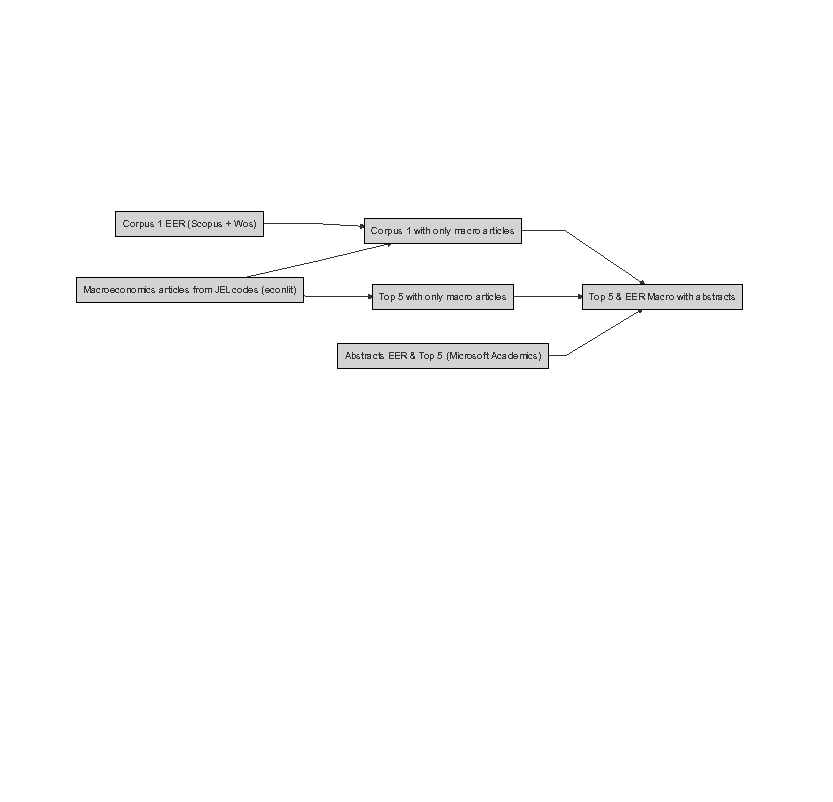
\includegraphics[width=1\linewidth]{First_version_files/figure-latex/plot-diagram-corpus-1} 

}

\caption{Construction of Corpus 2}\label{fig:plot-diagram-corpus}
\end{figure}

\hypertarget{b.2.-variable-creation}{%
\subsubsection*{B.2. Variable creation}\label{b.2.-variable-creation}}
\addcontentsline{toc}{subsubsection}{B.2. Variable creation}

\hypertarget{author-affiliation}{%
\paragraph*{Authors' affiliation}\label{author-affiliation}}
\addcontentsline{toc}{paragraph}{Authors' affiliation}

Authors' affiliations information were extracted from WoS. However, the
affiliations are not per author, but instead per institutional
departments per paper. For example, in the case of an article with two
authors from the same department, the department (and institution or
country associated with it) is only counted once. Similarly, a
single-authored article where the author has three affiliations can
result in one article having three affiliations. While in some cases we
can inferred the institutional affiliation for each author (e.g., one
institution, multiple authors), in others we cannot (e.g., two
institutions, three authors). For example, in an article with two
authors from Princeton and one author from Stanford, we only know that
the article was written by at least one author from Princeton and at
least one from Stanford, but not that the individual ratio was two
third.

We restructure the information in two ways.

First, for each article, we only kept one occurrence of each unique
institutions (university, research institutes\ldots) to avoid the
multiplication of observations resulting from the variety of departments
observed in some institutions. In other words, for each article, authors
are group by their institutional affiliation not by their department or
research team.

Second, and more importantly, for the purpose of our analysis, we mostly
looked at the share of papers authored by European-based and US-based
economists. While we do not have individual affiliation, we know with
certainty when a paper has only European authors, only American authors,
or a mix of the two. For this reason, while the share of institutions
within the corpus is only an estimation based on the occurrences of
affiliation, the information generated to identify US authored papers
and European authored paper is certain.

\hypertarget{network}{%
\subsubsection*{B.3. Bibliographic Coupling and Cluster
Detection}\label{network}}
\addcontentsline{toc}{subsubsection}{B.3. Bibliographic Coupling and
Cluster Detection}

A first way to identify potential differences between European and
American macroeconomics is to find articles written by Europeans and
published in European journals, resembling each others but dissimilar to
American articles. To do that, we used bibliographic coupling
techniques. In a bibliographic coupling network, a link is created
between two articles when they have one or more references in common.
The more references that two articles have in common, the stronger the
link. Bibliographic coupling is one way to measure how similar two
articles are in a corpus. To normalize and weight the link between two
articles, we used the refined bibliographic coupling strength of Shen et
al. (\protect\hyperlink{ref-shen2019}{2019}). This method normalized and
weight the strength between articles by taking into account two
important elements:

\begin{itemize}
\item
  the size of the bibliography of the two linked articles. It means that
  common references between two articles with long bibliography are
  weighted as less significant since the likeliness of potential common
  references is higher. Conversely, common references between two
  articles with a short bibliography is weighted as more significant.
\item
  the number of occurrences of each reference in the overall corpus.
  When a reference is shared between two articles, it is weighted as
  less significant if it is very common reference across the entire
  corpus and very significant if it is scarcely cited. The assumption is
  that a very rare common reference points to a higher content
  similarity between two articles than a highly cited reference.
\end{itemize}

For all macroeconomics articles published in the EER and in the Top 5,
we build the networks with 10-year overlapping windows. This results in
TO DO ALEX.

We used Leiden detection algorithm
(\protect\hyperlink{ref-traag2019}{Traag et al., 2019}) that optimize
the modularity on each network to identify groups of articles that are
similar to each others and dissimilar to the rest of the network. We use
a resolution of 1 with 1000 iterations. This results in TO DO ALEX
across all networks. Because networks have a lot of overlaps, many
clusters between two periods are composed of the same articles. To
identify these clusters that are very similar between two time windows,
we considered that \emph{(i)} if at least 55\% of the articles in a
community of the first time window where in the same cluster in the
second time window, and that \emph{(ii)} if the cluster was also
composed by at least 55\% of articles of the first time window,
\emph{then} it is the same cluster

Simply put, if two clusters share a high number of articles, and are
both mostly composed by these shared articles, they are considered the
same cluster.

This gives us TO DO ALEX, with TO DO ALEX that are at least 5\% of a
network at any given point and are stable enough to exists for at least
two time windows.

For each of these clusters, we computed the share of articles published
in the top 5 journals vs the EER, and the share of articles authored by
European vs American for the time window of the cluster We then
subtracted the share of articles published in the EER in the cluster
with the share of articles published in the EER on the same time period
of the cluster to identify over/under representation of the EER. We also
subtracted the relative share of European authors to American authors in
the cluster to the relative share of European authors to American on the
same time period of the cluster to identify over/under representation of
European authors in the cluster.

Finally, we plotted the clusters on a scatterplot to identify clusters
in which both European authors and the EER are over-represented.

\hypertarget{topic}{%
\subsubsection*{B.4. Topic Modelling}\label{topic}}
\addcontentsline{toc}{subsubsection}{B.4. Topic Modelling}

\hypertarget{preprocessing}{%
\paragraph*{Preprocessing}\label{preprocessing}}
\addcontentsline{toc}{paragraph}{Preprocessing}

We have several steps to clean our texts before running our topic
models:

\begin{enumerate}
\def\labelenumi{\arabic{enumi}.}
\tightlist
\item
  Once we have our corpus, we merge titles and abstracts together for
  all EER and Top 5 articles.
\item
  We use the \emph{tidytext} and \emph{tokenizers} R packages to
  `tokenise' the resulting texts (when there is no abstract, only the
  title if thus tokenise)?\footnote{See Silge J, Robinson D (2016).
    ``tidytext: Text Mining and Analysis Using Tidy Data Principles in
    R.'' \emph{JOSS}, \emph{1}(3) and Lincoln A. Mullen et al., ``Fast,
    Consistent Tokenization of Natural Language Text,'' Journal of Open
    Source Software 3, no.23 (2018): 655.} Tokenisation is the process
  of transforming human-readable text into machine readable objects.
  Here, the text is split in unique words (unigrams), bigrams (pair of
  words) and trigrams. In other words, to each article is now associated
  a list of unigrams, bigrams and trigrams, some appearing several times
  in the same title + abstract.
\item
  Stop words are removed using the \emph{Snowball}
  dictionary.\footnote{See
    http://snowball.tartarus.org/algorithms/english/stop.txt.} We add to
  this dictionary some current verbs in abstract like ``demonstrate'',
  ``show'', ``explain''. Such verbs are likely to be randomly
  distributed in abstracts, but we want to limit the noise as much as
  possible.
\item
  We lemmatise the words using the \emph{textstem} package.\footnote{Rinker,
    T. W. (2018). textstem: Tools for stemming and lemmatizing text
    version 0.1.4. Buffalo, New York.} The lemmatisation is the process
  of grouping words together according to their ``lemma'' which depends
  on the context. For instance, different form of a verb are reduced to
  its infinitive form. The plural of nouns are reduced to the singular.
\end{enumerate}

\hypertarget{choosing-the-number-of-topics}{%
\paragraph*{Choosing the number of
topics}\label{choosing-the-number-of-topics}}
\addcontentsline{toc}{paragraph}{Choosing the number of topics}

We use the Correlated Topic Model (\protect\hyperlink{ref-blei2007}{Blei
and Lafferty, 2007}) method implemented in the \emph{STM} R
package.\footnote{Roberts ME, Stewart BM, Tingley D (2019). ``stm: An R
  Package for Structural Topic Models.'' \emph{Journal of Statistical
  Software}, \emph{91}(2), 1-40.}

From the list of words we have tokenised, cleaned and lemmatised, we
test different thresholds and choices by running different models:

\begin{itemize}
\tightlist
\item
  by exluding trigrams or not;
\item
  by removing the terms that are present in less than 0.5\% of the
  Corpus (17), 1\% (34) and 2\% (68);
\item
  by removing articles with less than 6 words or with less than 12
  words.\footnote{Here, only articles with no abstract are impacted.}
\end{itemize}

Crossing all these criteria, we thus have 12 different possible
combinations. For each of these 12 different combinations, we have run
topic models for different number of topics from 20 to 110 with a gap of
5. The chosen model integrates trigram, removes only terms that appear
in less than 0,5\% of the documents and keep all articles if they have
more than 6 words in their title + abstract. We choose to keep the model
with 55 topics.

We have chosen the criteria and the number of topics by comparing the
performance of the different models in terms of the FREX value
(\protect\hyperlink{ref-bischof2012}{Bischof and Airoldi, 2012}).


\end{document}
